\documentclass[a4paper, 11pt, normalem]{report}

\usepackage{../../../LaTeX-Templates/Notes}
\usepackage{subfiles}

\newcommand\grint{\int_{z-\e}^{z+\e}}

\title{Mathematical Methods \\ In Physics \vspace{-20pt}}
\author{Dr Cristina Zambon and Fabrizio Caola}
\date{\vspace{-15pt}Michaelmas Term 2017 - Epiphany Term 2018}
\rhead{}

\begin{document}
\begin{titlepage}
    \newcommand{\HRule}{\rule{\linewidth}{0.5mm}}
    \center
    {
\includegraphics[scale=0.5]{../../logo0.png}\hfill{\Large\bfseries \shortstack{Michaelmas 2017 \\ - Epiphany 2018}}}\\[4cm]
    \HRule \\[0.7cm]
    {\huge\bfseries Mathematical Methods in Physics}\\[0.4cm]
    \HRule \\[1.5cm]

    \begin{minipage}{0.4\textwidth}
        \begin{flushleft} \large
            \emph{Author:} \\ Matthew Rossetter
        \end{flushleft}
    \end{minipage}~
    \begin{minipage}{0.4\textwidth}
        \begin{flushright} \large
            \emph{Lecturer:} \\ Prof. Cristina Zambon \\ Prof. Fabrizio Caola
        \end{flushright}
    \end{minipage}\\[2cm]
    \vfill
\end{titlepage}

\part{}
\chapter{}
\section{Geometrical Applications of Vectors in R3}
\begin{wrapfigure}{r}{0.4\textwidth}
    \begin{center}
        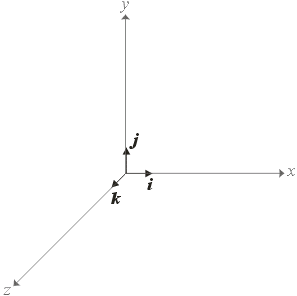
\includegraphics[scale=0.5]{Cart.png}
    \end{center}
\end{wrapfigure}
\begin{gather*}
    \vec{a} =
    \begin{pmatrix}
        a_1 \\
        a_2 \\
        a_3
    \end{pmatrix}
    \iff
    \vec{a} = a_{1}\hat{i} + a_{2}\hat{j} + a_{3}\hat{k} \\
    \vec{b} =
    \begin{pmatrix}
        b_1 \\
        b_2 \\
        b_3
    \end{pmatrix}
    \iff
    \vec{b} = b_{1}\hat{i} + b_{2}\hat{j} + b_{3}\hat{k}
\end{gather*}
We consider a Cartesian system:

$\{\hat{i}, \hat{j}, \hat{k}\} = $ 'standard basis'

This set is an orthonormal set of vectors:

The vectors $\hat{i}, \hat{j}, \& \hat{k}$ are orthogonal and have a modulus of 1

\begin{equation*}
    \hat{i} \perp \hat{j};~~ \hat{i} \perp \hat{k};~~ \hat{j} \perp \hat{k}
\end{equation*}
\begin{equation*}
    |\hat{i}| = |\hat{j}| = |\hat{k}| =  1
\end{equation*}

\section{Scalar (or dot) Product}
\begin{wrapfigure}{r}{0.35\textwidth}
    \begin{center}
        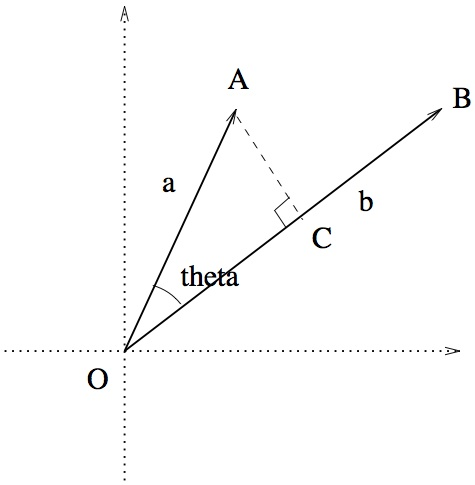
\includegraphics[scale=0.5]{Scalar.jpg}
    \end{center}
\end{wrapfigure}
\begin{gather*}
    \vec{a} \cdot \vec{b} = |\vec{a}||\vec{b}|\cos\theta \\
    \vec{a} \cdot \vec{b} = a_{1}b_{1} + a_{2}b_{2} + a_{3}b_{3}
\end{gather*}
$\vec{a}$ can be split into components $\perp$ and $\parallel$ to $\vec{b}$:
\begin{equation*}
    \vec{a} = \vec{a}_{\parallel} + \vec{a}_{\perp}
\end{equation*}
\begin{itemize}
    \item $\vec{a}_{\parallel} \equiv \vec{OC}$ is the orthogonal projection of $\vec{a}$ on to the direction of $\vec{b}$
    \item Its modulus is $|\vec{a}|\cos\theta = \frac{\vec{a} \cdot \vec{b}}{|\vec{a}|}$
\end{itemize}
\begin{equation*}
    \vec{a}_{\parallel} = \Bigg(\frac{\vec{a} \cdot \vec{b}}{|\vec{b}|}\Bigg) \frac{\vec{b}}{|\vec{b}|} \implies \vec{a}_{\perp} = \vec{a} - \vec{a}_{\parallel}
\end{equation*}
The dot product is symmetrical so:
\begin{gather*}
    \vec{a} \cdot \vec{b} = \vec{b} \cdot \vec{a} \\
    |\vec{a}| = \sqrt{\vec{a} \cdot \vec{a}}
\end{gather*}

\newpage
\section{Vector (or cross) Product}
\begin{wrapfigure}{r}{0.4\textwidth}
    \begin{center}
        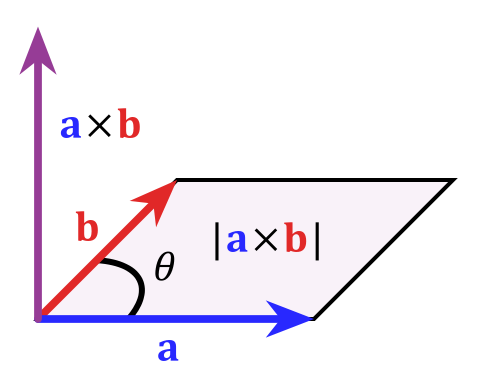
\includegraphics[scale=0.3]{Cross.png}
    \end{center}
    \vspace{-200pt}
\end{wrapfigure}
\begin{gather*}
    \vec{a} \times \vec{b} =
    \begin{pmatrix}
        a_1 \\
        a_2 \\
        a_3
    \end{pmatrix}
    \times
    \begin{pmatrix}
        b_1 \\
        b_2 \\
        b_3
    \end{pmatrix}
    =
    \begin{pmatrix}
        a_{2}b_{3} - a_{3}b_{2} \\
        a_{3}b_{1} - a_{1}b_{3} \\
        a_{1}b_{2} - a_{2}b_{1}
    \end{pmatrix} \\
    |\vec{a} \times \vec{b}| = |\vec{a}||\vec{b}|\sin\theta
\end{gather*}
Notice that $|\vec{a} \times \vec{b}|$ is the area of the parallelogram with sides $\vec{a}$ and $\vec{b}$

The cross product is anti-symmetric:
\begin{equation*}
    \vec{a} \times \vec{b} = -\vec{b} \times \vec{a}
\end{equation*}

\section{Scalar Triple Product}
\begin{equation*}
    [\vec{a}, \vec{b}, \vec{c}] = \vec{a} \cdot (\vec{b} \times \vec{c}) =
    \begin{vmatrix}
        a_1 & a_2 & a_3 \\
        b_1 & b_2 & b_3 \\
        c_1 & c_2 & c_3
    \end{vmatrix}
\end{equation*}
The absolute value of the scalar triple product for three arbitrary vectors $\vec{a}, \vec{b},$ and $\vec{c}$ corresponds to the volume of the parallelepiped with sides $\vec{a}, \vec{b},$ and $\vec{c}$
\begin{gather*}
    |[\vec{a}, \vec{b}, \vec{c}]| = |\vec{a}||\vec{b} \times \vec{c}|\cos\phi = |\vec{a}||\vec{b}||\vec{c}|\sin\theta\cos\phi
\end{gather*}
It is unchanged under an even permutation of the vectors:
\begin{equation*}
    [\vec{a}, \vec{b}, \vec{c}] = [\vec{b}, \vec{c}, \vec{a}] = [\vec{c}, \vec{a}, \vec{b}]
\end{equation*}
It changes sign under an odd permutation:
\begin{equation*}
    [\vec{a}, \vec{b}, \vec{c}] = -[\vec{b}, \vec{a}, \vec{c}] = -[\vec{a}, \vec{c}, \vec{b}] = -[\vec{c}, \vec{b}, \vec{a}]
\end{equation*}
It vanishes if any two vectors are the same

\section{Einstein Summation Convention for Subscripts}
\emph{Any index that appears twice in a given term of an expression is understood to be summed over all the values that an index can take}

The summed-over subscripts are called dummy subscripts and the others, free subscripts
\begin{gather*}
    \sum_{i = 1}^{n} a_{i}b_{i} \equiv a_{i}b_{i} \\
    a_{ij}b_{jk} = \sum_{j = 1}^{3} a_{ij}b_{jk} = a_{i1}b_{1k} + a_{i2}b_{2k} + a_{i3}b_{3k} \\
    a_{ij}b_{jk}c_{k} = \sum_{j = 1}^{3} \sum_{k = 1}^{3} a_{ij}b_{jk}c_{k} ~~~ \text{(Gives 9 terms)}
\end{gather*}

\section{Kronecker Delta in R3}
\begin{gather*}
    \delta_{ij} =
    \begin{cases}
        1 & \text{ if } i = j \\
        0 & \text{ otherwise}
    \end{cases}
    ;~~~ i,\,j = 1,\,2,\,3 \\
    b_{i}\delta_{ij} = b_{1}\delta_{1j} + b_{2}\delta_{2j} + b_{3}\delta_{3j}
    \begin{cases}
        j = 1 & \to ~ b_{1} \\
        j = 2 & \to ~ b_{2} \\
        j = 3 & \to ~ b_{3}
    \end{cases}
    \Bigg\} \implies b_{j} \\
    b_{i}\delta_{ij} = b_{j} \\
    \delta_{ii} = \delta_{11} + \delta_{22} + \delta_{33} = 3 \\
    \vec{a} \cdot \vec{b} = a_{i}b_{i} = \delta_{ij}a_{i}b_{j}
\end{gather*}

\section{Levi-Civita Symbol in R3}
\begin{gather*}
    \epsilon_{ijk} =
    \begin{cases}
        +1 & \text{if i,j,k is an even permutation of 1,2,3}       \\
           & \epsilon_{123} = \epsilon_{231} = \epsilon_{312} = 1  \\
        -1 & \text{if i,j,k is an odd permutation of 1,2,3}        \\
           & \epsilon_{213} = \epsilon_{132} = \epsilon_{321} = -1 \\
        0  & \text{otherwise}
    \end{cases}
\end{gather*}
\subsection{Features}
\begin{enumerate}
    \item $\epsilon_{ijk} = \epsilon_{jki}$ (even permutation) \\
          It does not change sign
    \item $\epsilon_{ijk} = -\epsilon_{jik}$ (odd permutation) \\
          It changes sign under the interchange of any pair of indices
    \item $\epsilon_{ijj} = \epsilon_{iii} = 0$
\end{enumerate}

\subsection{Exercises}
\begin{enumerate}
    \item $(\vec{a} \times \vec{b})_i = \epsilon_{ijk}a_{j}b_{k}$ \\
          $(\vec{a} \times \vec{b})_1 = \epsilon_{1jk}a_{j}b_{k} = \epsilon_{123}a_{2}b_{3} + \epsilon_{132}a_{3}b_{2} = a_{2}b_{3} - a_{3}b_{2}$
    \item $[\vec{a},\vec{b},\vec{c}] = \epsilon_{ijk}a_{i}b_{j}c_{k} =  a_{1}b_{2}c_{3} + a_{2}b_{3}c_{1} + a_{3}b_{1}c_{2} - a_{1}b_{3}c_{2} - a_{2}b_{1}c_{3} - a_{3}b_{2}c_{1}$
\end{enumerate}

\chapter{}
\section{Lines in R3}
\begin{wrapfigure}{r}{0.4\textwidth}
    \begin{center}
        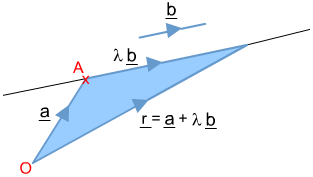
\includegraphics[scale=0.5]{EqLine.png}
    \end{center}
\end{wrapfigure}
Consider a point A and a direction $\hat{b}$:
\begin{gather*}
    (\vec{r} - \vec{a}) = \hat{b}\lambda \\
    \vec{r} = \vec{a} + \hat{b}\lambda
\end{gather*}
Note that $\vec{r} =\vec{r}(\lambda)$ (parametric form)

Note also that by taking the vector product with $\hat{b}$, we obtain another equation for the line:
\begin{equation*}
    (\vec{r} - \vec{a}) \times \hat{b} = 0
\end{equation*}

\section{Equation of a plane in R3}
\begin{wrapfigure}{r}{0.4\textwidth}
    \vspace{-20pt}
    \begin{center}
        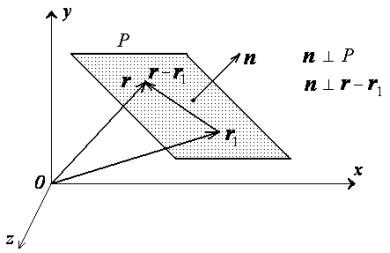
\includegraphics[scale=0.6]{Plane.jpg}
    \end{center}
    \vspace{-80pt}
\end{wrapfigure}
A plane through a point A with position vector, $\vec{a}$, and perpendicular to uni vector, $\hat{n}$, is:

\begin{gather*}
    (\vec{r} - \vec{a}) \cdot \hat{n} = 0 \\
    \vec{r} \cdot \hat{n} = \vec{a} \cdot \hat{n} = d
\end{gather*}
This is the Cartesian form for the equation of a plane

Consider a plane with points A, B, and C with corresponding position vectors:
\begin{equation*}
    t_{1}(\vec{b} - \vec{a}) + t_{2}(\vec{c} - \vec{a} = \vec{r} - \vec{a})
\end{equation*}
This is the parametric equation for a plane

\section{Linear Vector Spaces}
Found in Chapter 8 of Riley, Hobson, and Bence

A vector space, V, is a set whose elements are called "vectors" and such that there are two operations defined on them:
\begin{itemize}
    \item you can add vectors to each other
    \item you can multiply vectors by a scalar
\end{itemize}
Those operations must obey certain simple rules; these rules are called \emph{axioms} \\
The Axioms for a Vector Space are:
\begin{enumerate}
    \item The vector space is closed under addition and scalar multiplication
        \begin{itemize}
            \item If $\vec{v}$ and $\vec{u} \in$ V, then $\vec{v} + \vec{u} \in$ V
            \item If $\vec{v} \in$ V, then $\alpha\vec{v} \in$ V
        \end{itemize}
    \item Associativity
        \begin{itemize}
            \item $(\vec{u} + \vec{v}) + \vec{w} = \vec{u} + (\vec{v} + \vec{w})$
            \item $(\alpha\beta)\vec{v} = \alpha(\beta\vec{v})$
        \end{itemize}
    \item There exists a \emph{zero element} or \emph{neutral element}, $\vec{0}$
        \begin{itemize}
            \item $\vec{0} + \vec{v} = \vec{v}$
        \end{itemize}
    \item There exists an \emph{inverse element}, $-\vec{v}$
        \begin{itemize}
            \item $\vec{v} + (-\vec{v}) = \vec{0}$
        \end{itemize}
    \item Commutativity
        \begin{itemize}
            \item $\vec{u} + \vec{v} = \vec{v} + \vec{u}$
        \end{itemize}
    \item Distributivity
        \begin{itemize}
            \item $\alpha(\vec{v} + \vec{u}) = \alpha\vec{v} + \alpha\vec{u}$
            \item $(\alpha + \beta)\vec{v} = \alpha\vec{v} + \beta\vec{v}$
        \end{itemize}
    \item Scalar multiplication by 1 leaves $\vec{v}$ unchanged
        \begin{itemize}
            \item $1\vec{v} = \vec{v}$
        \end{itemize}
\end{enumerate}
Note that by scalar, we usually mean $\in \R$ \\
In this case, we refer to V as a \emph{real vector space}

It is also possible for scalars $\in \mathbb{C}$ \\
in this case, we have \emph{complex vector spaces}

\subsection{Examples}
\begin{enumerate}
    \item $\R$
    \item Generalisation to $\R^n$ for Euclidean vector spaces
    \item Further generalised to $\mathbb{C}^n$
    \item The set of all real functions, $f(x)$, with no restrictions on x and with the usual (calculus) addition and scalar multiplication
        \begin{itemize}
            \item $(f_1 + f_2 )(x) = f_{1}(x) + f_{2}(x)$
            \item $(\alpha f)(x) = \alpha f(x)$
        \end{itemize}
    \item The matrices of size $(n \times m)$ with real elements and the usual (calculus) addition and scalar multiplication of matrices
    \item The set of vectors in the 3D space for which $2X - 3Y + 11Z + 2 = 0$ \textbf{is not a vector space}
        \begin{itemize}
            \item $\vec{0} \notin$ V
            \item $2\cdot0 - 3\cdot0 + 11\cdot0 + 2 \neq 0$
        \end{itemize}
    \item $2X - 3Y + 11Z = 0$ is a vector space
    \item Consider a second order, linear, homogeneous differential equation of the form:
        \begin{itemize}
            \item $p(x)\frac{d^{2}f}{dx^2} + q(x)\frac{df}{dx} + r(x)f = 0$
            \item p, q, and r are fixed functions
        \end{itemize}
        The space of the solutions of such an equation forms a vector space under the usual addition and scalar multiplication
\end{enumerate}

\chapter{}
For k vectors, $\{\vec{v}_{1},\vec{v}_{2},\cdots,\vec{v}_{k}\}$ in V, the expression $\{\alpha_{1}\vec{v}_{1},\alpha_{2}\vec{v}_{2},\cdots,\alpha_{k}\vec{v}_{k}\}$ is called a linear combination.

The set of all linear combinations of $\{\vec{v}_{1},\vec{v}_{2},\cdots,\vec{v}_{k}\}$ is called a span of $\{\vec{v}_{1},\vec{v}_{2},\cdots,\vec{v}_{k}\}$:
\begin{equation*}
    \text{Span}(\vec{v}_{1},\cdots,\vec{v}_{n}) = \Bigg\{\sum_{i = 1}^{k} \alpha_{i}\vec{v}_{i} ~;~ \alpha_{i} \in \R / \mathbb{C} \Bigg\}
\end{equation*}

\section{Examples}
\begin{enumerate}
    \item A span of a single vector is the set of all scalar multiples of this vector
        \begin{itemize}
            \item it is a line through 0 in the direction of the vector
        \end{itemize}
    \item The span of two vectors, provided they are not multiples of each other, can be seen as the plane through 0 containing these vectors
\end{enumerate}

\section{Definition}
A set of vectors, $\{\vec{v}_{1},\vec{v}_{2},\cdots,\vec{v}_{k}\} \in V$ is called linearly independent if
\begin{equation*}
    \sum_{i = 1}^{k} \alpha_{i}\vec{v}_{i} = 0 \implies \alpha_{i} = 0 ~\forall~ i
\end{equation*}
Otherwise, the vectors are called linearly dependent \\
That is, these vectors are linearly dependent if
\begin{equation*}
    \sum_{i = 1}^{k} \alpha_{i}\vec{v}_{i} = 0 \implies \alpha_{i} \neq 0 \text{ for one }i
\end{equation*}

\subsection{Claim}
The vectors $\{\vec{v}_{1},\vec{v}_{2},\cdots,\vec{v}_{k}\}$ are linearly dependent $\iff \vec{v}_{i}$ can be written as a linear combination of the other vectors

\subsection{Examples}
\begin{enumerate}
    \item   \begin{gather*}
                \vec{v}_{1} =
                \begin{pmatrix}
                    0 \\
                    1 \\
                    1
                \end{pmatrix}
                ~;~
                \vec{v}_{2} =
                \begin{pmatrix}
                    0 \\
                    1 \\
                    2
                \end{pmatrix}
                ~;~
                \vec{v}_{3} =
                \begin{pmatrix}
                    1 \\
                    1 \\
                    -1
                \end{pmatrix} \\
                \alpha_{1}\vec{v}_{1} + \alpha_{2}\vec{v}_{2} + \alpha_{3}\vec{v}_{3} =
                \begin{pmatrix}
                    \alpha_{3} \\
                    \alpha_{1} + \alpha_{2} + \alpha_{3} \\
                    \alpha_{1} + 2\alpha_{2} - \alpha_{3}
                \end{pmatrix} = 0 \\
                \alpha_{3} = 0 ~;~ \alpha_{1} = -\alpha_{2} ~;~ \alpha_{1} = \alpha_{2} = 0 \\
                \text{These vectors are linearly independent}
            \end{gather*}
    \item   \begin{gather*}
                \vec{v}_{1} =
                \begin{pmatrix}
                    -2 \\
                    0  \\
                    1
                \end{pmatrix} ~;~
                \vec{v}_{2} =
                \begin{pmatrix}
                    1 \\
                    1 \\
                    1
                \end{pmatrix} ~;~
                \vec{v}_{3} =
                \begin{pmatrix}
                    0 \\
                    2 \\
                    3
                \end{pmatrix} \\
                \alpha_{1}\vec{v}_{1} + \alpha_{2}\vec{v}_{2} + \alpha_{3}\vec{v}_{3} =
                \begin{pmatrix}
                    -2\alpha_{1} + \alpha_{2} \\
                    \alpha_{2} + 2\alpha_{3}  \\
                    \alpha_{1} + \alpha_{2} + 3\alpha_{3}
                \end{pmatrix} = 0 \\
                \alpha_{1} = 1 ~;~ \alpha_{2} ~;~ \alpha_{3} = -1 \\
                \text{These vectors are linearly dependent}
            \end{gather*}
            Notice that $\vec{v}_{3} = \vec{v}_{1} + 2\vec{v}_{2}$ \\
            Can calculate linear dependence using determinant:
            \begin{equation*}
                det(\vec{v}_{1},\vec{v}_{2},\vec{v}_{3}) = 0 \implies \text{linearly dependent}
            \end{equation*}
    \item   The set of polynomials of degree 2 or less with coefficients in $\R$ form a vector space \\
    Consider these three polynomials:
            \begin{gather*}
                \Bigg\{\underbrace{1 + x + x^2}_{\vec{v}_1} ~;~ \underbrace{1 - x + 3x^2}_{\vec{v}_2} ~;~ \underbrace{1 + 3x - x^2}_{\vec{v}_3} \Bigg\} \\
                \alpha_{1}\vec{v}_{1} + \alpha_{2}\vec{v}_{2} + \alpha_{3}\vec{v}_{3} = \alpha_{1}(1 + x + x^2) + \alpha_{1}(1 - x + 3x^2) + \alpha_{3}(1 + 3x - x^2) = 0 \\
                x^{2}\underbrace{(\alpha_{1} + 3\alpha_2 - \alpha_3)}_{0} + x\underbrace{(\alpha_1 - \alpha_2 + 3\alpha_3)}_{0} + \underbrace{(\alpha_1 + \alpha_2 + \alpha_3)}_{0} = 0 \\
                \alpha_1 = -2\alpha_2 ~;~ \alpha_3 = \alpha_2 ~;~ \alpha_2 = n,~n \in \R \\
                \vec{v}_3 = 2\vec{v}_1 - \vec{v}_2
            \end{gather*}
\end{enumerate}

\section{Definition}
The minimal set of vectors that span a vector space is called a basis for that space.

A set of vectors $\{\vec{v}_{1},\vec{v}_{2},\cdots,\vec{v}_{k}\} \in V$ is called a basis $\iff$
\begin{enumerate}
    \item $\{\vec{v}_{1},\vec{v}_{2},\cdots,\vec{v}_{k}\}$ are linearly independent
    \item $V = \text{Span}(\{\vec{v}_{1},\vec{v}_{2},\cdots,\vec{v}_{k}\})$
\end{enumerate}

Then we have that:
\begin{itemize}
    \item The number of vectors in a basis is the dimension of a vector space
    \item If $\{\vec{v}_{1},\vec{v}_{2},\cdots,\vec{v}_{k}\}$ is a basis in V, any $\vec{v}_n \in V$ can be written as a unique linear combination of the vectors in the basis, $\vec{v}_n = \alpha_i \vec{v}_i$
        \begin{itemize}
            \item Coefficients $\alpha_i$ are called the components of $\vec{v}$ wrt to the basis
        \end{itemize}
\end{itemize}

\subsection{Examples}
\begin{enumerate}
    \item Previous example 2(i). It is a basis in $\R^3$ (dim 3)
    \item For the 2x3 matrices with entries $\R$, a basis is given by:
            \begin{gather*}
                E_{11} =
                \begin{pmatrix}
                    1 & 0 & 0 \\
                    0 & 0 & 0
                \end{pmatrix} ~;~
                E_{12} =
                \begin{pmatrix}
                    0 & 1 & 0 \\
                    ) & 0 & 0
                \end{pmatrix} \text{etc} \\
                E_{ij},~ i = 1,2 ~;~ j = 1,2,3
            \end{gather*}
    \item Polynomials of degree 2 or less with coefficients in $\R$ \\
          Basis is:
            \begin{gather*}
                \Bigg\{1 ~;~ x ~;~ x^2 \Bigg\} ~\text{(dim 3)}
            \end{gather*}
\end{enumerate}

\section{Inner (or scalar) product}
Consider a vector space, V \\
The inner product of V is a scalar function denoted $\langle \vec{v} \mid \vec{w} \rangle$ that satisfies the following properties:
\begin{enumerate}
    \item $\langle \vec{v} \mid \vec{w} \rangle = \langle \vec{w} \mid \vec{v} \rangle^*$
    \item $\langle \vec{v} \mid \alpha\vec{w} + \beta\vec{u} \rangle = \alpha\langle \vec{v} \mid \vec{w} \rangle + \beta\langle \vec{v} \mid \vec{u} \rangle$
    \item $\langle \vec{v} \mid \vec{v} \rangle > 0,~ \vec{v} \neq 0$
\end{enumerate}
Notes:
\begin{itemize}
    \item Two vectors are orthogonal if $\langle \vec{v} \mid \vec{w} \rangle = 0$
    \item Length of a vector (norm) is $|\vec{v}| = \sqrt{\langle \vec{v} \mid \vec{v} \rangle}$
\end{itemize}

\subsection{Examples}
\begin{enumerate}
    \item In $\R$, the dot product:
            \begin{gather*}
                \langle \vec{v} \mid \vec{w} \rangle = \vec{v}^{\dagger} \cdot \vec{w} =
                \begin{pmatrix}
                    v_1 & v_2 & v_3
                \end{pmatrix}
                \begin{pmatrix}
                    w_1 \\
                    w_2 \\
                    w_3
                \end{pmatrix} \\
                \implies v_{1}w_{1} + v_{2}w_{2} + v_{3}w_{3}
            \end{gather*}
    \item In $\mathbb{C}$:
            \begin{gather*}
                \langle \vec{v} \mid \vec{w} \rangle = \vec{v}^{\dagger} \cdot \vec{w} = (\vec{v}^{\,T})^{*} \cdot \vec{w} =
                \begin{pmatrix}
                    v_{1}^{*} & v_{2}^{*} & v_{3}^{*}
                \end{pmatrix}
                \begin{pmatrix}
                    w_1 \\
                    w_2 \\
                    w_3
                \end{pmatrix} \\
                \implies v_{1}^{*}w_{1} + v_{2}^{*}w_2 + v_{3}^{*}w_3 = v_{i}^{*}w_i
                \implies |\vec{v}| = \sqrt{\langle \vec{v} \mid \vec{v} \rangle} = \sqrt{\vec{v}^{\,T} \cdot \vec{v}} \\
                \text{E.g.} \\
                \vec{v} =
                \begin{pmatrix}
                    1 \\
                    0 \\
                    i
                \end{pmatrix} \implies |\vec{v}| =
                \sqrt{  \begin{pmatrix}
                            1 & 0 & -i
                        \end{pmatrix}
                        \begin{pmatrix}
                            1 \\
                            0 \\
                            i
                        \end{pmatrix}} = \sqrt{1 + 1} = \sqrt{2}
            \end{gather*}
\end{enumerate}

\chapter{}
\section{Matrices}
From now on, we work in $\R$ or $\mathbb{C}$

\subsection{Definition}
\emph{An operator is an object that associates a vector to another vector}
\begin{enumerate}
    \item Matrices are good examples of operators:
            \begin{equation*}
                A\bar{a} = \bar{b} ~;~ A_{ij}a_j = b_i
            \end{equation*}
          $A_{ij}$ is an element of the matrix, A
    \item Matrices are linear operators
            \begin{gather*}
                \mathbf{A}(\bar{a} + \bar{b}) = \mathbf{A}\bar{a} + \mathbf{A}\bar{b} \\
                \mathbf{A}(\alpha\bar{a}) = \alpha \mathbf{A}\bar{a}
            \end{gather*}
\end{enumerate}

\section{Operators with Matrices}
\begin{enumerate}
    \item Matrix addition and matrix multiplication \\
          Note that matrix multiplication is not commutative: $\mathbf{AB} \neq \mathbf{BA}$
    \item The transpose of a matrix:
            \begin{gather*}
                (\mathbf{A^{T}})_{ij} = \mathbf{A}_{ji} \\
                \mathbf{(ABCD)^T} = \mathbf{D^{T}C^{T}B^{T}A^{T}}
            \end{gather*}
    \item The complex conjugation of a matrix:
            \begin{gather*}
                (\mathbf{A}^{*})_{ij} = (\mathbf{A}_{ij})^*
            \end{gather*}
    \item The Hermitian conjugate of a matrix: (adjoint)
            \begin{equation*}
                (\mathbf{A}^{\dagger})_{ij} = (\mathbf{A}_{ij})^{\dagger}
            \end{equation*}
    \item The trace of a square matrix: \\
          \textit{It is the sum of diagonal elements}
          \begin{equation*}
              \text{Tr}(\mathbf{A}) = \mathbf{A}_{ii}
          \end{equation*}
          Notice that the trace is invariant under cyclic permutations, i.e.
          \begin{gather*}
              \text{Tr}(\mathbf{AB}) = \text{Tr}(\mathbf{BA}) \\
              \text{Tr}(\mathbf{ABC}) = \text{Tr}(\mathbf{BCA}) = \text{Tr}(\mathbf{CAB})
          \end{gather*}
    \item The inverse of a square matrix: \\
          The inverse of a matrix, $\mathbf{A}$, is a matrix denoted by $\mathbf{A}^{-1}$ such that $\mathbf{AA^{-1}} = \mathbf{A^{-1}A} = \mathbf{I}$
          \begin{flalign*}
              &\text{Identity Matrix:} &\mathbf{I}_{ij} &= \delta_{ij}&
          \end{flalign*}
          Note that a matrix, $\mathbf{A}$, could not have an inverse. If $\nexists ~\mathbf{A}^{-1}$, then matrix $\mathbf{A}$ is said to be singular
\end{enumerate}

\subsection{Properties of the Inverse}
\begin{enumerate}
    \item   \begin{gather*}
                \mathbf{(ABCD)^{-1}} = \mathbf{D^{-1}C^{-1}B^{-1}A^{-1}}
            \end{gather*}
    \item   \begin{gather*}
                (\mathbf{A^T})^{-1} = (\mathbf{A^{-1}})^T
            \end{gather*}
\end{enumerate}
The most straight-forward way for calculating the inverse of a matrix is the \emph{Gauss-Jordan method}.

This uses \emph{Elementary Row Operations}:
\begin{itemize}
    \item Multiply any row by a non-zero constant
    \item Interchange any two rows
    \item Add some multiple of one row to another
\end{itemize}

\subsection{Example}
\begin{gather*}
    A =
    \begin{pmatrix}
        1 & 2 & 4 \\
        1 & 3 & 5 \\
        2 & 2 & 7
    \end{pmatrix}. ~~
    \text{Find the inverse of }\mathbf{A} \text{ if it exists.} \\
    \text{Use an augmented matrix of }\mathbf{A|\,I}: \\
    \begin{array}{ccc|ccc}
        1 & 2 & 4 & 1 & 0 & 0 \\
        1 & 3 & 5 & 0 & 1 & 0 \\
        2 & 2 & 7 & 0 & 0 & 1
    \end{array} \implies
    \begin{array}{ccc|ccc}
        1 &  2 &  4 &  1 & 0 & 0 \\
        0 &  1 &  1 & -1 & 1 & 0 \\
        0 & -2 & -1 & -2 & 0 & 1 \\
    \end{array} \implies
    \begin{array}{ccc|ccc}
        1 & 2 & 4 &  1 & 0 & 0 \\
        0 & 1 & 1 & -1 & 1 & 0 \\
        0 & 0 & 1 & -4 & 2 & 1
    \end{array} \implies \\
    \begin{array}{ccc|ccc}
        1 & 0 & 2 &  3 & -2 & 0 \\
        0 & 1 & 1 & -1 &  1 & 0 \\
        0 & 0 & 1 & -4 &  2 & 1
    \end{array} \implies
    \begin{array}{ccc|ccc}
        1 & 0 & 0 & 11 & -6 & -2 \\
        0 & 1 & 0 &  3 & -1 & -1 \\
        0 & 0 & 1 & -4 &  2 &  1
    \end{array} \implies \\
    \mathbf{A}^{-1} =
    \begin{pmatrix}
        11 & -6 & -2 \\
         3 & -1 & -1 \\
        -4 &  2 &  1
    \end{pmatrix}
\end{gather*}

\section{Determinant of a square matrix}
\subsection{Definition}
The minor $\mathbf{|A_{ij}|}$ associated with element $\mathbf{A_{ij}}$ of a $(n \times m)$ matrix, $\mathbf{A}$, is the determinant of the $(n - 1) \times (n - 1)$ matrix obtained by removing all elements in the $i$th row and the $j$th column
\begin{equation*}
    |\mathbf{A}| = \text{det}(\mathbf{A}) = \mathbf{A_{11}|A_{11}|} - \mathbf{A_{12}|A_{12}|} + \mathbf{A_{13}|A_{13}|} \cdots + (-1)^{m - 1} \mathbf{A_{1m}|A_{1m}|}
\end{equation*}
This is called the Laplace expansion along the first column \\
The Laplace expansion can be performed along any row or column

\subsection{Example}
\begin{enumerate}
    \item   \begin{gather*}
                \mathbf{A} =
                \begin{pmatrix}
                    \mathbf{A_{11}} & \mathbf{A_{12}} \\
                    \mathbf{A_{21}} & \mathbf{A_{22}}
                \end{pmatrix} \\
                \mathbf{|A|} = \mathbf{A_{11}A_{22}} - \mathbf{A_{12}A_{21}}
            \end{gather*}
    \item   \begin{gather*}
                \mathbf{A} =
                \begin{pmatrix}
                    \mathbf{A_{11}} & \mathbf{A_{12}} & \mathbf{A_{13}} \\
                    \mathbf{A_{21}} & \mathbf{A_{22}} & \mathbf{A_{23}} \\
                    \mathbf{A_{31}} & \mathbf{A_{32}} & \mathbf{A_{33}}
                \end{pmatrix} \\
                \mathbf{|A|} = \mathbf{A_{11}}
                \begin{vmatrix}
                    \mathbf{A_{22}} & \mathbf{A_{23}} \\
                    \mathbf{A_{32}} & \mathbf{A_{33}}
                \end{vmatrix} - \mathbf{A_{12}}
                \begin{vmatrix}
                    \mathbf{A_{21}} & \mathbf{A_{23}} \\
                    \mathbf{A_{31}} & \mathbf{A_{33}}
                \end{vmatrix} + \mathbf{A_{13}}
                \begin{vmatrix}
                    \mathbf{A_{21}} & \mathbf{A_{22}} \\
                    \mathbf{A_{31}} & \mathbf{A_{32}}
                \end{vmatrix} \\
                \mathbf{|A|} = (\mathbf{A_{11}A_{22}A_{33}} + \mathbf{A_{12}A_{23}A_{31}} + \mathbf{A_{13}A_{21}A_{32}}) - (\mathbf{A_{11}A_{23}A_{32}} + \mathbf{A_{12}A_{21}A_{33}} + \mathbf{A_{13}A_{22}A_{31}}) \\
                \mathbf{|A|} = \mathbf{A_{1i}A_{2j}A_{3k}}\epsilon_{ijk}
            \end{gather*}
\end{enumerate}

\subsection{Properties of the Determinant}
\begin{enumerate}
    \item $$\mathbf{|ABCD|} = \mathbf{|A||B||C||D|} ~~ (\mathbf{|AB|} = \mathbf{|BA|})$$
    \item   \begin{gather*}
                \mathbf{|A|^T} = \mathbf{|A|} ~;~ \mathbf{|A^{*}|} = \mathbf{|A|^*} ~;~ \mathbf{|A^{\dagger}|} = \mathbf{|A|^*} \\
                \mathbf{|A^{-1}|} = \mathbf{|A|^{-1}} \implies \mathbf{|A|} = 0 \to \nexists~ \mathbf{A^{-1}}
            \end{gather*}
    \item If two rows or columns are linearly dependent, then: $$\mathbf{|A|} = 0$$
    \item If $\mathbf{B}$ is obtained from $\mathbf{A}$ by interchanging two rows or columns then:
            \begin{gather*}
                \mathbf{|B|} = -\mathbf{|A|}
            \end{gather*}
    \item If $\mathbf{B}$ is obtained from $\mathbf{A}$ by multiplying the elements of any row or column by $\alpha$, then:
            \begin{gather*}
                \mathbf{|B|} = \alpha\mathbf{|A|} \\
                \mathbf{B} = \alpha\mathbf{A} \implies \mathbf{|B|} = \alpha^k \mathbf{|A|} ~;~ \text{k is number of rows or columns}
            \end{gather*}
\end{enumerate}

\chapter{}
\section{The Eigenvalue Problem}
Consider an $(n \times n)$ matrix. We want to answer the following question:

Are there any vectors $\bar{x} = 0$ which are transformed by $\mathbf{A}$ into multiples of themselves,
\begin{equation*}
    \mathbf{A}\bar{x} = \lambda\bar{x}
\end{equation*}
If it exists, $\bar{x}$ is an eigenvector, and $\lambda$ is its eigenvalue

$(\mathbf{A} - \lambda\mathbf{I})\bar{x} = 0$ represents a set of homogeneous linear equations \\
Such a set of equations will only have a non-trivial solution set if $|\mathbf{A} - \lambda\mathbf{I}| = 0$

\subsection{Definition}
$|\mathbf{A} - \lambda\mathbf{I}| = 0$ is called the characteristic equation, or polynomial of degree n

The eigenvalues, $\lambda$, are the n solutions of this equation

\subsection{Example}
Construct the characteristic equation, $|\mathbf{A} - \lambda\mathbf{I}| = 0$:
\begin{gather*}
    \mathbf{A} =
    \begin{pmatrix}
        1 & 2 & 1 \\
        2 & 1 & 1 \\
        1 & 1 & 2
    \end{pmatrix} \\
    \begin{vmatrix}
        1 - \lambda &           2 &           1 \\
                  2 & 1 - \lambda &           1 \\
                  1 &           1 & 2 - \lambda \\
    \end{vmatrix} = 0 \\
    \cdots \implies \\
    \lambda = 1,4,-1
\end{gather*}
For $\lambda = 1$, solve $(\mathbf{A} - \mathbf{I})\bar{x} = 0$
\begin{gather*}
    \begin{pmatrix}
        0 & 2 & 1 \\
        2 & 0 & 1 \\
        1 & 1 & 1
    \end{pmatrix}
    \begin{pmatrix}
        x_1 \\
        x_2 \\
        x_3
    \end{pmatrix} \implies
    \begin{matrix*}
        2x_2 + x_3 = 0 \\
        2x_1 + x_3 = 0 \\
        x_1 + x_2 + x_3 = 0
    \end{matrix*} \\
    \bar{x} =
    \begin{pmatrix}
          x_1 \\
          x_1 \\
        -2x_1
    \end{pmatrix} \to e.g.~ \bar{x} =
    \begin{pmatrix}
         1 \\
         1 \\
        -2
    \end{pmatrix} \implies \hat{x} = \frac{1}{\sqrt{6}}
    \begin{pmatrix}
         1 \\
         1 \\
        -2
    \end{pmatrix}
\end{gather*}
Can repeat for other $\lambda$s

Note that eigenvectors are generally linearly dependent \\
Eigenvectors are mutually orthogonal in special cases

If a $(n \times n)$ matrix, $\mathbf{A}$, has n distinct eigenvalues, then the set of corresponding eigenvectors represent a basis in the vector space on which the matrix acts

If the eigenvectors are not all distinct (i.e. degenerate), the basis may or may not exist

If $\mathbf{A}$ has zero eigenvalues, then $\mathbf{A}$ must be singular $\implies |\mathbf{A} - \lambda\mathbf{I}| = |\mathbf{A}| = 0$

\subsection{Example}
\begin{gather*}
    \mathbf{A} =
    \begin{pmatrix}
        -2 &  2 & -3 \\
         2 &  1 & -6 \\
        -1 & -2 &  0
    \end{pmatrix} \implies |\mathbf{A} - \lambda\mathbf{I}| =
    \begin{vmatrix}
        -2 - \lambda &           2 &       -3 \\
                   2 & 1 - \lambda &       -6 \\
                  -1 &          -2 & -\lambda
    \end{vmatrix} = 0 \\
    \lambda^3 + \lambda^2 -21\lambda - 45 = 0 \implies \lambda = 5,-3,-3
\end{gather*}
Degenerate eigenvalue of $-3$

For $\lambda = 5$, solve $(\mathbf{A} - 5\mathbf{I}) = 0$:
\begin{gather*}
    \bar{x} =
    \begin{pmatrix}
         1 \\
         2 \\
        -1
    \end{pmatrix}
\end{gather*}
For $\lambda_2 = \lambda_3 = -3$, solve $(\mathbf{A} + 3\mathbf{I}) = 0$:
\begin{gather*}
    \begin{pmatrix}
         1 &  2 & -3 \\
         2 &  4 & -6 \\
        -1 & -2 &  3
    \end{pmatrix}
    \begin{pmatrix}
        x_1 \\
        x_2 \\
        x_3
    \end{pmatrix} \implies
    \begin{matrix}
         x_1 + 2x_2 - 3x_3 = 0 \\
        2x_1 + 4x_2 - 6x_3 = 0 \\
        -x_1 - 2x_2 + 3x_3 = 0
    \end{matrix} \Bigg\}\; same \;equation \\
    x_1 = -2x_2 + 3x_3 \implies \bar{x} =
    \begin{pmatrix}
        -2x_2 + 3x_3 \\
                 x_2 \\
                 x_3
    \end{pmatrix}
\end{gather*}
This yields linearly independent eigenvectors

\section{Special Matrices}
\begin{enumerate}
    \item Symmetric Matrix: $\mathbf{A} = \mathbf{A^T}$
    \item Hermitian Matrix: $\mathbf{A} = \mathbf{A^{\dagger}}$
    \item[] \textbf{Theorem:} The eigenvalues of an Hermitian or Symmetric matrix are real
    \item Antisymmetric Matrix: $\mathbf{A^T} = -\mathbf{A}$
    \item Anti-Hermitian Matrix: $\mathbf{A^{\dagger}} = -\mathbf{A}$
    \item[] \textbf{Theorem:} The eigenvalues of an Antisymmetric or Anti-Hermitian matrix are purely imaginary or zero
    \item Orthogonal Matrix: $\mathbf{A^T} = \mathbf{A^{-1}} \implies \mathbf{A^{T}A} = \mathbf{I}$
    \item Unitary Matrix: $\mathbf{A^{\dagger}} = \mathbf{A^{-1}} \implies \mathbf{A^{\dagger}A} = \mathbf{I}$
    \item[] \textbf{Theorem:} The eigenvalues of an Unitary or Orthogonal matrix have unit modulus, i.e $|\lambda|^{2} = 1$
\end{enumerate}

\chapter{}
\section{Special Matrices Continued}
\subsection{Theorem - Eigenvalues of a Hermitian or Symmetric Matrix are real}
\vspace{-20pt}
\begin{alignat*}{3}
    \mathbf{A}\bar{x} &= \lambda\bar{x} \quad& \implies \quad& \bar{x}\mathbf{A^{\dagger}} &= \lambda^{*}\bar{x}^{\dagger} \\
    & \Downarrow \quad& \implies \quad& \bar{x}^{\dagger}\mathbf{A} &= \lambda^{*}\bar{x}^\dagger \\
    \bar{^\dagger}\mathbf{A}\bar{x} &= \lambda\bar{x}^\dagger \bar{x} \quad& \& \quad& \bar{x}^\dagger \bar{x} &= \lambda^{*}\bar{x}^\dagger \bar{x} \\
    (\lambda^{*} - \lambda)&\bar{x}^{\dagger}\bar{x} = 0 \quad& \lambda^* = \lambda \quad& &\lambda \in \R
\end{alignat*}

\subsection{Theorem - Eigenvectors of special matrices are linearly independent}
In addition, they can be chosen such that they are mutually orthogonal
\vspace{-15pt}
\textbf{Definition}
Two matrices, $\mathbf{A}$ and $\mathbf{A}'$, are said to be similar if $\mathbf{A}' = \mathbf{S^{-1}AS}$ (similarity transformation)

$\mathbf{A}$ and $\mathbf{A}'$ represent the same linear operator in different bases \\
These bases are related by $\mathbf{S}$ \\
$\mathbf{A}$ and $\mathbf{A}'$ share a few basis-independent properties:
\begin{enumerate}
    \item $\mathbf{|A|} = \mathbf{|A'|}$
    \item $\text{Tr}(\mathbf{A}) = \text{Tr}(\mathbf{A'})$
    \item $\{\lambda s \,of\, \mathbf{A}\} = \{ \lambda s \,of\, \mathbf{A}'\}$
\end{enumerate}

\section{Diagonalisation of a Matrix}
If the new basis is chosen to be a set of eigenvectors of $\mathbf{A}$, then the matrix $\mathbf{A}' = \mathbf{D}$ is diagonal
\begin{gather*}
    \mathbf{D} = \mathbf{S^{-1}AS} \\
    \mathbf{D} =
    \begin{pmatrix}
        \lambda_1 & & & \\
        & \lambda_2 & & \\
        & & \ddots &    \\
        & & & \lambda_n
    \end{pmatrix} ~;~ \mathbf{S}
    \begin{pmatrix}
        \vdots & \vdots & & \vdots \\
        \bar{x}_1 & \bar{x}_2 & \cdots & \bar{x}_n \\
        \vdots & \vdots & & \vdots \\
        \vdots & \vdots & & \vdots
    \end{pmatrix} \\
    \begin{aligned}
        \mathbf{AS} &=& \mathbf{A}
        \begin{pmatrix}
            \vdots & \vdots & & \vdots \\
            \bar{x}_1 & \bar{x}_2 & \cdots & \bar{x}_n \\
            \vdots & \vdots & & \vdots \\
            \vdots & \vdots & & \vdots
        \end{pmatrix} \\ &=&
        \begin{pmatrix}
            \vdots & \vdots & & \vdots \\
            \mathbf{A}\bar{x}_1 & \mathbf{A}\bar{x}_2 & \cdots & \mathbf{A}\bar{x}_n \\
            \vdots & \vdots & & \vdots \\
            \vdots & \vdots & & \vdots
        \end{pmatrix} \\ &=&
        \begin{pmatrix}
            \vdots & \vdots & & \vdots \\
            \lambda_{1}\bar{x}_1 & \lambda_{2}\bar{x}_2 & \cdots & \lambda_{n}\bar{x}_n \\
            \vdots & \vdots & & \vdots \\
            \vdots & \vdots & & \vdots
        \end{pmatrix} \\ &=&
        \begin{pmatrix}
            \vdots & \vdots & & \vdots \\
            \bar{x}_1 & \bar{x}_2 & \cdots & \bar{x}_n \\
            \vdots & \vdots & & \vdots \\
            \vdots & \vdots & & \vdots
        \end{pmatrix} \mathbf{D}
    \end{aligned} \\
    \mathbf{AS} = \mathbf{SD} \\
    \mathbf{D} = \mathbf{S^{-1}AS}
\end{gather*}
\begin{enumerate}
    \item $\mathbf{|A|} = \mathbf{|D|} = \prod_{i = 1}^{n} \lambda_i = \lambda_{1} \times \lambda_{2} \times \cdots \times \lambda_{n}$
    \item $\text{Tr}(\mathbf{A}) = \text{Tr}(\mathbf{D}) = \sum_{i = 1}^{n} \lambda_i = \lambda_1 + \lambda_2 + \cdots + \lambda_n$
\end{enumerate}

\subsection{Example}
\begin{gather*}
    \mathbf{A} =
    \begin{pmatrix}
        5 & 4 \\
        1 & 2
    \end{pmatrix} \implies
    \begin{aligned}
        \lambda_1 &= 6 & \lambda_2 &= 1 \\
        \bar{x}_1 &=
        \begin{pmatrix}
            4 \\
            1
        \end{pmatrix} & \bar{x}_2 &=
        \begin{pmatrix}
            1 \\
            -1
        \end{pmatrix}
    \end{aligned} \\
    \begin{aligned}
        \mathbf{D} &=
        \begin{pmatrix}
            6 & 0 \\
            0 & 1
        \end{pmatrix} & \mathbf{S} &=
        \begin{pmatrix}
            4 & 1 \\
            1 & -1
        \end{pmatrix} & \mathbf{S^{-1}} &= \frac{1}{5}
        \begin{pmatrix}
            1 & 1 \\
            1 & -4
        \end{pmatrix}
    \end{aligned} \\
    \text{Tr}(\mathbf{A}) = 7 = \mathbf{D} \\
    \mathbf{|A|} = 6 = \mathbf{|D|}
\end{gather*}
Consider special matrices \\
Since it is always possible to find a basis of eigenvectors, then these matrices are always diagonisable.

Since the eigenvectors can be chosen to be an orthonormal set then the matrix $\mathbf{S}$ becomes unitary, i.e. $\mathbf{D} = \mathbf{S^{-1}AS}$ becomes $\mathbf{D} = \mathbf{S^{\dagger}AS} ~ (S^{-1} = S^{\dagger})$

For an orthonormal set, $\{\bar{x}_1, \bar{x}_2, \cdots, \bar{x}_n\} \to \underline{\bar{x}_i \cdot \bar{x}_j = \delta_{ij}},~~ \mathbf{S^{\dagger}S} = \mathbf{I}$

\begin{align*}
    \mathbf{S^{\dagger}S} &=
    \begin{pmatrix}
        \cdots & \bar{x}_{1}^* & \cdots & \cdots \\
        \cdots & \bar{x}_{2}^* & \cdots & \cdots \\
               & \vdots        &        &        \\
        \cdots & \bar{x}_{n}^* & \cdots & \cdots
    \end{pmatrix}
    \begin{pmatrix}
        \vdots & \vdots & & \vdots \\
        \bar{x}_1 & \bar{x}_2 & \cdots & \bar{x}_n \\
        \vdots & \vdots & & \vdots \\
        \vdots & \vdots & & \vdots
    \end{pmatrix} \\ &=
    \begin{pmatrix}
        \bar{x}_{1}^{\dagger}\bar{x}_{1} & \bar{x}_{1}^{\dagger}\bar{x}_{2} & \cdots & \bar{x}_{1}^{\dagger}\bar{x}_{n} \\
        \bar{x}_{2}^{\dagger}\bar{x}_{1} & \cdots & & \vdots \\
        \vdots & \ddots & & \vdots \\
        \bar{x}_{n}^{\dagger}\bar{x}_{1} & \cdots & \cdots & \bar{x}_{n}^{\dagger}\bar{x}_{n}
    \end{pmatrix} \\ &=
    \begin{pmatrix}
        1 & 0 & \cdots & 0 \\
        0 & \cdots & & \vdots \\
        \vdots & \ddots & & \vdots \\
        0 & \cdots & \cdots & 1
    \end{pmatrix} = (\delta_{ij}) &
\end{align*}

\subsection{Example}
For a symmetric matrix:
\begin{gather*}
    \begin{aligned}
        A &=
        \begin{pmatrix}
            1  & 0 & 3 \\
            0 & -2 & 0 \\
            3 &  0 & 1
        \end{pmatrix} & \lambda_1 &= 4 & \lambda_{2/3} &= -2 \\ \bar{x}_1 &=
        \begin{pmatrix}
            a \\
            0 \\
            a
        \end{pmatrix} & \bar{x}_{2/3} &=
        \begin{pmatrix}
            b \\
            c \\
            -b
        \end{pmatrix} \\
        \bar{x}_1 &= \frac{1}{\sqrt{2}}
        \begin{pmatrix}
            1 \\
            0 \\
            1
        \end{pmatrix} & \bar{x}_2 &= \frac{1}{\sqrt{2}}
        \begin{pmatrix}
            1 \\
            0 \\
            -1
        \end{pmatrix} & \bar{x}_3 &=
        \begin{pmatrix}
            0 \\
            1 \\
            0
        \end{pmatrix} \\ \mathbf{S} &= \frac{1}{\sqrt{2}}
        \begin{pmatrix}
            1 & 1 & 0 \\
            0 & 0 & \sqrt{2} \\
            1 & -1 & 0
        \end{pmatrix} & \mathbf{S^{\dagger}} &= \frac{1}{\sqrt{2}}
        \begin{pmatrix}
            1 & 0 & 1 \\
            1 & 0 & -1 \\
            0 & \sqrt{2} & 0
        \end{pmatrix}
    \end{aligned} \\
    \mathbf{D} =
    \begin{pmatrix}
        4 & 0 & 0 \\
        0 & -2 & 0 \\
        0 & 0 & -2
    \end{pmatrix} = \frac{1}{2}
    \begin{pmatrix}
        1 & 0 & 1 \\
        1 & 0 & -1 \\
        0 & \sqrt{2} & 0
    \end{pmatrix}
    \begin{pmatrix}
        1 & 0 & 3 \\
        0 & -2 & 0 \\
        3 & 0 & -1
    \end{pmatrix}
    \begin{pmatrix}
        1 & 1 & 0 \\
        0 & 0 & \sqrt{2} \\
        1 & -1 & 0
    \end{pmatrix} = \mathbf{S^{\dagger}AS}
\end{gather*}

\section{Application: Power of Matrices}
\begin{gather*}
    \mathbf{A}^n = \underbrace{\mathbf{AA \cdots A}}_{\text{n times}} \text{ if } \mathbf{D} = \mathbf{S^{-1}AS} \text{ then } \\
    \begin{aligned}
        \mathbf{A} = \mathbf{SDS^{-1}} \implies \mathbf{A}^n &= (\mathbf{SDS^{-1}})^n \\
        &= \underbrace{(\mathbf{SDS^{-1}})(\mathbf{SDS^{-1}})\cdots(\mathbf{SDS^{-1}})}_{\text{n times}} \\
        &= \mathbf{SD^nS^{-1}}
    \end{aligned} \\
    \mathbf{D}^n =
    \begin{pmatrix}
        \lambda_{1}^n & & & \\
        & \lambda_{2}^n & & \\
        & & \ddots & \\
        & & & \lambda_{n}^n
    \end{pmatrix}
\end{gather*}

\chapter{}
\section{Fourier Series (FS)}
FS are series of $\cos$ and $\sin$ - trig series

They are used to represent periodic functions \\
A function f(x) is called periodic if $f(x + l) = f(x) ~\forall~ x$ \\
$l > 0$, called the period

The Fourier expansion of a periodic function, f(x), with period L is:
\begin{align*}
    f(x) &= \frac{a_0}{2} + \sum_{r = 1}^{\infty} \Bigg[a_r \cos\Big(\frac{2\pi rx}{L}\Big) + b_r \sin\Big(\frac{2\pi rx}{L}\Big)\Bigg] \\
    a_r &= \frac{2}{L} \int_{x_0}^{x_0 + L} f(x)\cos\Big(\frac{2\pi rx}{L}\Big)\,dx,~ r = 0,1,2,\cdots \\
    b_r &= \frac{2}{L} \int_{x_0}^{x_0 + L} f(x)\sin\Big(\frac{2\pi rx}{L}\Big)\,dx,~ r = 1,2,3,\cdots
\end{align*}
$x_0$ is arbitrary since the integral is a function with period L

FS are infinite sums so need to be sure they converge

An FS converges if f(x) satisfies the \underline{Dirichlet Conditions}

\section{Dirichlet Conditions}
In the interval L, the periodic function f(x)
\begin{enumerate}
    \item is single-valued $\forall~ x_0 \leq x \leq x_0 + L$
    \item has a finite number of finite discontinuities
    \item has a finite number of extreme values, i.e. maxima and minima
        \begin{itemize}
            \item This implies that we can represent non-continuous functions by FS
        \end{itemize}
\end{enumerate}
The set of all periodic functions on the interval L that can be represented by FS forms a Vector Space:
\begin{enumerate}
    \item Operation: Standard addition and scalar multiplication
    \item Basis:
            \begin{align*}
                1 && \sin\Big(\frac{2\pi rx}{L}\Big) && \cos\Big(\frac{2\pi rx}{L}\Big) && r > 0
            \end{align*}
        \begin{itemize}
            \item Infinite number of elements, i.e. infinite dimension vector space
        \end{itemize}
    \item A general element of the space can be written as a linear combination of the basis elements:
            \begin{equation*}
                f(x) = \frac{a_0}{2} \cdot 1 + \sum_{r = 1}^{\infty} \Bigg[a_r \cos\Big(\frac{2\pi rx}{L}\Big) + b_r \sin\Big(\frac{2\pi rx}{L}\Big)\Bigg]
            \end{equation*}
    \item Inner product: $\langle f \,|\, g \rangle$
            \begin{equation*}
                \langle f \,|\, g \rangle = \frac{2}{L} \int_{0}^{L} f(x)g(x)\,dx \\
            \end{equation*}
            The basis is orthogonal so:
            \begin{align*}
                \langle f \,|\, g \rangle &= \frac{2}{L} \Bigg[ \\
                & \int_{0}^{L} \sin\Big(\frac{2\pi rx}{L}\Big)\cos\Big(\frac{2\pi px}{L}\Big) \, dx = 0 \\
                &+ \int_{0}^{L} \sin\Big(\frac{2\pi rx}{L}\Big)\sin\Big(\frac{2\pi px}{L}\Big) \, dx =
                \begin{cases}
                    0 & r \neq p \\
                    \frac{L}{2} & r = p
                \end{cases} \\
                &+ \int_{0}^{L} \cos\Big(\frac{2\pi rx}{L}\Big)\cos\Big(\frac{2\pi px}{L}\Big) \, dx =
                \begin{cases}
                    0 & r \neq p \\
                    \frac{L}{2} & r = p > 0 \\
                    L & r = p = 0
                \end{cases} \Bigg]
            \end{align*}
\end{enumerate}
\begin{itemize}
    \item  If f(x) is even, i.e. $f(-x) = f(x)$, then $b_r = 0 ~\forall~ r \in \mathbb{N}$
    \item If f(x) is odd, i.e. $f(-x) = -f(x)$, then $a_r = 0 ~\forall~ r \in \mathbb{N}$
\end{itemize}

\subsection{Example}
A function in the interval of $-\pi \leq x \leq \pi$:
\begin{gather*}
    f(x) =  \begin{cases}
                -x & -\pi \leq x \leq 0 \\
                x & 0 \leq x \leq \pi
            \end{cases} \\
    L = 2\pi
\end{gather*}
f(x) is even so $b_r = 0$
\begin{align*}
    a_r &= \frac{1}{\pi} \int_{-\pi}^{0} (-x)\cos(rx) \, dx + \frac{1}{\pi} \int_{0}^{\pi} x\cos(rx) \, dx \\
    & = \frac{2}{\pi} \int_{0}^{\pi} x\cos(rx) \, dx
\end{align*}
Could choose the interval of $0 \leq x \leq 2\pi$ instead for the same function
\begin{align*}
    f(x) &= \begin{cases}
                x & 0 \leq x \leq \pi \\
                2\pi - x & \pi \leq x \leq 2\pi
            \end{cases} \\
    a_r &= \frac{1}{\pi} \int_{0}^{\pi} x\cos(rx) \, dx + \frac{1}{\pi} \int_{\pi}^{2\pi} (2\pi - x)\cos(rx) \, dx \\
    &=
    \begin{cases}
        a_r = \frac{2}{\pi} \frac{(-1)^r - 1}{r^2} & r > 0 \\
        a_0 = \pi &
    \end{cases}
\end{align*}

\subsection{Example}
\begin{gather*}
    f(x) =  \begin{cases}
                -1 & -\pi < x < 0 \\
                1 & 0 < x < \pi
            \end{cases}
    L = 2\pi
\end{gather*}
f(x) is odd so $a_r = 0$
\begin{align*}
    b_r &= \frac{1}{\pi} \int_{0}^{\pi} \sin(rx) \, dx - \frac{1}{\pi} \int_{-\pi}^{0} \sin(rx) \, dx \\
    &= \frac{2}{\pi} \sin(rx) \, dx = \frac{2}{r\pi} (1 - (-1)^r),~ r > 0 \\
    b_r &=  \begin{cases}
                0 & r \text{ even} \\
                \frac{4}{r\pi} & r \text{ odd}
            \end{cases} \\
    f(x) &= \frac{4}{\pi} \sum_{r = 1}^{\infty} \frac{\sin((2r - 1)x)}{2r - 1}\\
         &= \frac{4}{\pi} \Big(\sin(x) + \frac{\sin(3x)}{3} + \cdots \Big)
\end{align*}
Function at $x = n\pi$ is discontinuous - the value of the FS at these values is zero

The sum of the FS at a jump (discontinuity), $x_0$, is equal to the average of the two function values on either side, i.e.
\begin{equation*}
    \frac{1}{2}\big[f(x_{0}^-) + f(x_{0}^+) \big]
\end{equation*}

\chapter{}
\section{FS Continued}
Sometimes we have functions that are defined only on a finite interval. In order to calculate the FS for this, we need to extend the function by means of functions that are periodic.

\subsection{Example}
\begin{equation*}
    f(x) = x^2,~ 0 \leq x \leq 2
\end{equation*}
In order to calculate FS, we need to think of possible extensions:
\begin{enumerate}
    \item Extend to $x^2,~ -2 \leq x \leq 2$ - this is even and continuous
    \item   \begin{gather*}
                f(x) =  \begin{cases}
                            x^2 & 0 \leq x < 2 \\
                            -x^2 & -2 < x \leq 0
                        \end{cases}
            \end{gather*}
            This is odd and non-continuous
    \item Extend as $x^2,~ 0 < x < 2$ - this is non-continuous
\end{enumerate}
All these extensions are fine in the sense that they are a fine representation of the function $f(x) = x^2,~ 0 \leq x \leq 2$

However, they have a different value at $x = 2$ \\
In general, continuous extensions are preferable - Gibb's phenomenon at points of discontinuity

FS evaluated at specific points can be used to calculate series of constant terms \\
Consider Example 2 in Lecture 7:
\begin{align*}
    f(x) &= \begin{cases}
                -1 & -\pi < x < 0 \\
                1 & 0 < x < \pi
            \end{cases} \\
    f(x) &= \frac{4}{\pi} \Big(\sin x + \frac{\sin 3x}{3} + \frac{\sin 5x}{5} + \cdots \Big)
\end{align*}
Choose $f(x = \frac{\pi}{2}) = 1$:
\begin{align*}
    f(x = \frac{\pi}{2}) &= \frac{4}{\pi} (\sin \frac{\pi}{2} + \cdots) \\
    1 &= \frac{4}{\pi} \Big(1 - \frac{1}{3} + \frac{1}{5} -\frac{1}{7} + \cdots \Big) \\
    \frac{\pi}{4} &= 1 - \frac{1}{3} + \frac{1}{5} -\frac{1}{7} + \cdots \\
    &= \sum_{n = 0}^{\infty} (-1)^n \frac{1}{2n + 1}
\end{align*}

\section{Calculus of FS}
\begin{enumerate}
    \item If we integrate a FS with respect to x, we get a power of r at the denominator of each coefficient. This results in a more rapid convergence, meaning a FS can always be integrated.
    \item If we differentiate a FS with respect to x, we get a power of r at the numerator of each coefficient. This reduces the rate of convergence, so must be careful with differentiation.
\end{enumerate}

\subsection{Example}
Consider $f(x) = x^2,~ 0 \leq x \leq 2$ \\
In order to write FS, we need a periodic function

Let's choose the even one looked at previously ($b_r = 0$):
\begin{align*}
    f(x) &= x^2,~ 2 \leq x \leq 2,~ L = 4 \\
    f(x) &= \frac{4}{3} + 16\sum_{r = 1}^{\infty} \frac{(-1)^r}{(\pi r)^2}\cos\Big(\frac{\pi rx}{2}\Big) \equiv x^2,~ 0 \leq x \leq 2
\end{align*}
This FS represents the function $f(x) = x^2,~ 0 \leq x \leq 2$

\section{Integrating FS}
\begin{align*}
    \int \frac{4}{3}dx + 16\sum_{r = 1}^{\infty} \frac{(-1)^r}{(\pi r)^2} \int \cos\Big(\frac{\pi rx}{2}\Big)\,dx &= \int x^2 dx \\
    \frac{4}{3}x + 32\sum_{r = 1}^{\infty} \frac{(-1)^r}{(\pi r)^3}\sin\Big(\frac{\pi rx}{2}\Big) + C &= \frac{1}{3}x^3
\end{align*}
This is not a FS - C and $\frac{4}{3}x$ are not in terms of $\sin$ and $\cos$

\section{Differentiating FS}
\begin{align*}
    \frac{d}{dx}\bigg(\frac{4}{3}\bigg) + 16\sum_{r = 1}^{\infty} \frac{(-1)^r}{(\pi r)^2} \frac{d}{dx}\bigg(\cos\Big(\frac{\pi rx}{2}\Big)\bigg) &= \frac{d}{dx}\bigg(x^2\bigg) \\
    -8 \sum_{r = 1}^{\infty} \frac{(-1)^r}{\pi r} \sin\Big(\frac{\pi rx}{2}\Big) &= 2x \\
    \implies -4\sum_{r = 1}^{\infty} \frac{(-1)^r}{\pi r} \sin\Big(\frac{\pi rx}{2}\Big) &= x
\end{align*}
Use this result in the integrated expression to resolve issues:
\begin{align*}
    -16\sum_{r = 1}^{\infty} \frac{(-1)^r}{\pi r} \sin\Big(\frac{\pi rx}{2}\Big) + 96\sum_{r = 1}^{\infty} \frac{(-1)^r}{(\pi r)^3}\sin\Big(\frac{\pi rx}{2}\Big) + C' &= x^3
\end{align*}
Almost have a FS for $g(x) = x^3,~ 0 \leq x \leq 2$
\begin{align*}
    g(0) = 0 \implies& C' = 0 \\
    -16\sum_{r = 1}^{\infty} \frac{(-1)^r}{\pi r} \sin\Big(\frac{\pi rx}{2}\Big) + 96\sum_{r = 1}^{\infty} \frac{(-1)^r}{(\pi r)^3}\sin\Big(\frac{\pi rx}{2}\Big) &= x^3
\end{align*}
This is the FS of $g(x) = x^3,~ 0 \leq x \leq 2$

\section{Complex FS}
The FS's can be written in complex form:
\begin{align*}
    f(x) &= \frac{a_0}{2} + \sum_{r = 1}^{\infty} \bigg(a_r \cos\Big(\frac{2\pi rx}{L}\Big) + b_r \sin\Big(\frac{2\pi rx}{L}\Big)\bigg) \\
    &= \frac{a_0}{2} + \sum_{r = 1}^{\infty} \Bigg(\frac{a_r}{2}\bigg(e^{i\tfrac{2\pi rx}{L}} + e^{-i\tfrac{2\pi rx}{L}}\bigg) + \frac{b_r}{2i}\bigg(e^{i\tfrac{2\pi rx}{L}} - e^{-i\tfrac{2\pi rx}{L}} \bigg)\Bigg) \\
    &= \frac{a_0}{2} + \sum_{r = 1}^{\infty} \Bigg(e^{i\tfrac{2\pi rx}{L}} \Big(\frac{a_r}{2} + \frac{b_r}{2i}\Big) + e^{-i\tfrac{2\pi rx}{L}}\Big(\frac{a_r}{2} - \frac{b_r}{2i}\Big)\Bigg)
\end{align*}
\begin{gather*}
    \frac{a_r - b_r i}{2} \equiv c_r ~;~ \frac{a_r + b_r i}{2} \equiv d_r \\
    a_r = a_{-r} ~;~ b_r = b_{-r} \\
    d_r = c_{-r}
\end{gather*}
\begin{align*}
    f(x) &= \frac{a_0}{2} + \sum_{r = 1}^{\infty} \bigg(c_r e^{i\tfrac{2\pi rx}{L}} + c_{-r}e^{-i\tfrac{2\pi rx}{L}}\bigg) \\
    &= \sum_{-\infty}^{\infty} c_r e^{i\tfrac{2\pi rx}{L}},~ c_0 = \frac{a_0}{2}
\end{align*}

\chapter{}
\section{Integral Transforms}
A function $g(y)$ defined by the equation
\begin{equation*}
    g(y) = \ifnt k(x,y)f(x)\,dx = I[f(x)](y)
\end{equation*}
is called the integral transform of $f(x)$
\begin{enumerate}
    \item The function $k(x,y)$ is called the kernel of the transform
    \item I is linear, i.e.
            \begin{equation*}
                I[c_1 f_1 + c_2 f_2] = c_1 I[f_1] + c_2 I[f_2]
            \end{equation*}
    \item If I is given, can introduce the inverse, $I^-1$, such that
            \begin{equation*}
                I[f] = g \to I^{-1}[g] = f
            \end{equation*}
\end{enumerate}
There are several types of ITs. Consider the Fourier and the Laplace transforms

\section{Fourier Transforms (FTs)}
FT of f is defined by
\begin{equation*}
    \mathcal{F}[f(t)](\om) = \hat{f}(\om) = \frac{1}{\sqrt{2\pi}}\ifnt f(t)\underbrace{e^{-i\om t}}_{k(x,y)}dt
\end{equation*}
The integral exists if:
\begin{enumerate}
    \item f has a finite number of finite discontinuities
    \item $\ifnt |f(t)|\,dt$ is finite, i.e. it converges
\end{enumerate}
If f is continuous, can define the inverse FT as
\begin{equation*}
    \mathcal{F}^{-1}[\hat{f}(\om)](t) = f(t) = \frac{1}{\sqrt{2\pi}} \ifnt \hat{f}(\om) e^{i\om t}d\om
\end{equation*}
There are different forms for the FTs:
\begin{enumerate}
    \item   \begin{equation*}
                \hat{f}(\om) = \ifnt f(t)e^{-i\om t}dt ~;~ f(t) = \frac{1}{2\pi} \ifnt \hat{f}(\om)e^{i\om t}d\om
            \end{equation*}
    \item   \begin{equation*}
                \hat{f}(\om) = \frac{1}{\sqrt{2\pi}} \ifnt f(t)e^{i\om t}dt ~;~ f(t) = \frac{1}{\sqrt{2\pi}} \ifnt \hat{f}(\om)e^{-i\om t}d\om
            \end{equation*}
    \item   \begin{equation*}
                \om = 2\pi v \to \hat{f}(v) = \ifnt f(t)e^{-i2\pi vt}dt ~;~ f(t) = \ifnt \hat{f}(v) e^{i2\pi vt}dv
            \end{equation*}
\end{enumerate}
There are functions that are not periodic, therefore, cannot use FS for them. Can imagine that these functions are defined over an infinite interval.

Consider complex FS:
\begin{align*}
    f(t) &= \ifsum c_n e^{i\tfrac{2\pi nt}{L}} = \ifsum \Bigg(\frac{1}{L}\int_{-\tfrac{L}{2}}^{\tfrac{L}{2}} f(t)e^{-i\tfrac{2\pi nt}{L}}dt \Bigg)e^{i\tfrac{2\pi nt}{L}} \\
    \frac{2\pi n}{L} &= \om_n \implies \Delta \om = \om_{n + 1} - \om_n = \frac{2(n + 1)\pi}{L} - \frac{2\pi n}{L} = \frac{2\pi}{L} \\
    f(t) &= \ifsum \Bigg(\frac{\Delta \om}{2\pi} \int_{-\tfrac{L}{2}}^{\tfrac{L}{2}} f(t)e^{-it\om_n}dt\Bigg) e^{it\om_n}
\end{align*}
As $L \to \infty$:
\begin{itemize}
    \item   \begin{equation*}
                \Big[-\frac{L}{2},\frac{L}{2}\Big] \to (-\infty, \infty)
            \end{equation*}
    \item   \begin{equation*}
                \om_n \to \om
            \end{equation*}
    \item   \begin{equation*}
                \Delta \om \to d\om
            \end{equation*}
    \item   \begin{equation*}
                \ifsum \to \ifnt
            \end{equation*}
\end{itemize}
\begin{align*}
    f(t) &= \ifnt \frac{d\om}{\sqrt{2\pi}}\underbrace{\Bigg(\ifnt \frac{1}{\sqrt{2\pi}} f(t)e^{-i\om t} dt\Bigg)}_{\hat{f}(\om)} e^{i\om t}
\end{align*}
\begin{table}[H]
    \centering
    \begin{tabular}{|c|c|}
        \hline
            Fourier Series &     Fourier Transforms \\
        \hline
        Periodic functions & Non-periodic functions \\
             Finite period &        Infinite period \\
         Discrete spectrum &    Continuous spectrum \\
        \hline
    \end{tabular}
\end{table}

\subsection{Example}
\begin{align*}
    f(t) &=
    \begin{cases}
        0 & -\frac{L}{2} < t < -\frac{a}{2} \\
        1 & -\frac{a}{2} < t < \frac{a}{2}  \\
        0 & \frac{a}{2} < t < \frac{L}{2}
    \end{cases} \\
    f(t) &= f(t + L)
\end{align*}
FS is complex:
\begin{align*}
    c_n &= \frac{a}{L} \frac{\sin\big(\tfrac{n\pi a}{L}\big)}{\tfrac{n\pi a}{L}} \\
    f(t) &= \ifsum \frac{a}{L} \frac{\sin\big(\tfrac{n\pi a}{L}\big)}{\tfrac{n\pi a}{L}} e^{i\tfrac{2\pi nt}{L}}
\end{align*}
The $c_n$, called the spectral coefficient of the $n^{th}$ harmonic, form a discrete complex spectrum
\begin{equation*}
    |c_n| \approx |\frac{\sin t_n}{t_n}|
\end{equation*}
As the period increases, the separation between the pulses increases as well. In the limit, $L \to \infty$, only a single pulse remains and the resulting function is:
\begin{equation*}
    f(t) =
    \begin{cases}
        1 & -\frac{a}{2} < t < \frac{a}{2} \\
        0 & \text{otherwise}
    \end{cases}
\end{equation*}
This is non-periodic \\
The FT is:
\begin{align*}
    \hat{f}(\om) &= \frac{1}{\sqrt{2\pi}} \ifnt f(t)e^{-i\om t}dt = \frac{1}{\sqrt{2\pi}} \int_{-\tfrac{a}{2}}^{\tfrac{a}{2}} e^{-i\om t}dt \\
    &= \frac{1}{\sqrt{2\pi}} \Bigg[\frac{e^{-i\om t}}{-i\om} \Bigg]_{-\tfrac{a}{2}}^{\tfrac{a}{2}} = \frac{2}{\sqrt{\pi}} \frac{1}{-2i\om} \Big(e^{-i\tfrac{\om a}{2}} - e^{i\tfrac{\om a}{2}}\Big) \\
    &= \frac{a}{\sqrt{2\pi}} \frac{\sin\big(\tfrac{a\om}{2}\big)}{\tfrac{a\om}{2}}
\end{align*}

\chapter{}
\section{Fourier Transforms Continued}
\begin{align*}
    \F[f(t)](\om) &= \hat{f}(\om) = \frac{1}{\sqrt{2\pi}} \ifnt f(t)e^{-i\om t}dt \\
    \F^{-1}[\hat{f}(\om)](t) &= f(t) = \frac{1}{\sqrt{2\pi}} \ifnt \hat{f}(\om)e^{i\om t}d\om
\end{align*}

\subsection{Properties}
\begin{itemize}
    \item Scaling
            \begin{align*}
                \F[f(at)](\om) &= \frac{1}{\sqrt{2\pi}} \ifnt f(at)e^{-i\om t}dt, ~(at = t') \\
                &= \frac{1}{|a|} \F[f(t')]\Big(\frac{\om}{a}\Big) = \frac{1}{|a|\sqrt{2\pi}} \ifnt f(t') e^{-i\om \tfrac{t'}{a}}dt' \\
                &= \frac{1}{|a|} \hat{f}\Big(\frac{\om}{a}\Big)
            \end{align*}
    \item Transposition
            \begin{equation*}
                \F[f(t + a)](\om) = e^{i\om a} \F[f(t)](\om) = e^{i\om a}\hat{f}(\om)
            \end{equation*}
    \item Exponential Multiplication
            \begin{equation*}
                \F[e^{at}f(t)](\om) = \F[f(t)](\om + ia) = \hat{f}(\om + ia)
            \end{equation*}
\end{itemize}
\subsection{Example}
\begin{align*}
    \F\Big[f\big(\frac{t}{2}\big)\cos(\alpha t)\Big](\om) &= \frac{1}{2}\F\Big[f\big(\frac{t}{2}\big)e^{i\alpha t}\Big](\om) + \frac{1}{2}\F[f\big(\frac{t}{2}\big)e^{-i\alpha t}](\om) \\
    &= \frac{1}{2}\cdot2 \F[f(t)e^{2i\alpha t}](2\om) + \frac{1}{2}\cdot2 \F[f(t)e^{-2i\alpha t}](2\om) \\
    &= \F[f(t)](2\om - 2\alpha) + \F[f(t)](2\om + 2\alpha)
\end{align*}

\section{Fourier Transform of a Derivative (differential rule)}
\begin{align*}
    \F[f'(t)](\om) &= i\om \hat{f}(\om) \\
    \F[f''(t)](\om) &= -\om^2 \hat{f}(\om) \\
    \F[f^{(n)}(t)](\om) &= (i\om)^n \hat{f}(\om)
\end{align*}

\section{Convolution}
The convolution of two functions is defined as
\begin{equation*}
    h(y) = \ifnt f(x)g(y - x)\,dx = (f \star g)(y) = (g \star f)(y)
\end{equation*}

\section{Convolution Theorem}
The FT of the convolution $h(y)$ is the product of the FTs of f and g:
\begin{align*}
    \hat{h}(k) &= \sqrt{2\pi} \hat{f}(k) \hat{g}(k) \\
    \hat{h}(k) &= \frac{1}{\sqrt{2\pi}} \ifnt h(y)e^{-iyk}dy = \frac{1}{\sqrt{2\pi}} \ifnt \Bigg(\ifnt f(x)g(y - x)\,dx\Bigg)e^{-iyk}dy \\
    &= \frac{1}{\sqrt{2\pi}} \ifnt f(x) \Bigg(\ifnt g(y - x)e^{-iyk}dy\Bigg)\,dx, ~ (y - x = z) \\
    &= \frac{1}{\sqrt{2\pi}} \ifnt f(x) \Bigg(\ifnt g(z)e^{-i(z + x)k}dz\Bigg)\,dx \\
    &= \frac{1}{\sqrt{2\pi}} \ifnt f(x)e^{-ixk}dx \Bigg(\frac{1}{\sqrt{2\pi}}\sqrt{2\pi} \ifnt g(z)e^{-izk}dz \Bigg) \\
    &= \sqrt{2\pi} \hat{f}(k) \hat{g}(k)
\end{align*}

\subsection{Example}
\begin{equation*}
    \frac{d^2 f}{dt^2} + 2\frac{df}{dt} + f(t) = h(t)
\end{equation*}
Apply FT on both sides:
\begin{gather*}
    \F\Big[\frac{d^2 f}{dt^2}\Big](\om) + 2\F\Big[\frac{df}{dt}\Big](\om) + \F[f(t)](\om) = \F[h(t)](\om) \\
    -\om^2 \hat{f}(\om) + 2i\om \hat{f}(\om) + \hat{f}(\om) = \hat{h}(\om) \\
    \begin{aligned}
        \hat{f}(\om) &= \frac{\hat{h}(\om)}{(1 + 2i\om - \om^2)} \\
        &= \frac{\hat{h}(\om)}{(i\om + 1)^2}
    \end{aligned}
\end{gather*}
\begin{enumerate}
    \item   \begin{equation*}
                f(t) = \F^{-1}\Bigg[\frac{\hat{h}(\om)}{(i\om + 1)^2}\Bigg]
            \end{equation*}
    \item   \begin{align*}
                \hat{f}(\om) &= \frac{\hat{h}(\om)}{(i\om + 1)^2} = \sqrt{2\pi}\hat{h}(\om) \hat{g}(\om),~~ \Big[\hat{g}(\om) = \frac{1}{\sqrt{2\pi}} \frac{1}{(i\om + 1)^2} \\
                f(t) &= \ifnt g(t')h(t - t')\,dt'
            \end{align*}
\end{enumerate}

\section{Dirac delta-function}
Consider a pulse,
\begin{equation*}
    \delta_n (x) =  \begin{cases}
                        n & -\tfrac{1}{2n} < x < \tfrac{1}{2n} \\
                        0 & \text{otherwise}
                    \end{cases}
\end{equation*}
If we take the duration of the pulse to decrease while at the same time retaining a unit area, then in the limit, we are lead to the notion of the Dirac $\delta$-function:
\begin{align*}
    \lim_{n \to \infty} \ifnt \delta_n (x)\,dx &= \ifnt \delta(x)\,dx = 1 \\
    \lim_{n \to \infty} \ifnt \delta_n (x) f(x)\,dx &= \ifnt \delta(x)f(x)\,dx = f(0)
\end{align*}
$\delta$-function is not a standard function. It is a generalised function distribution. \\
It is defined as the limit of a sequence of functions (not a unique sequence)

Its defining properties are:
\begin{enumerate}
    \item   \begin{equation*}
                \delta(x - a) = 0,~ x \neq a
            \end{equation*}
    \item   \begin{equation*}
                \int_{\alpha}^{\beta} f(x)\delta(x - a)\,dx =
                \begin{cases}
                    f(a) & \alpha < a < \beta \\
                    0 & \text{otherwise}
                \end{cases}
            \end{equation*}
\end{enumerate}

\section{Example}
\begin{enumerate}
    \item   \begin{equation*}
                \int_{-4}^{4} \delta(x - \pi)\cos(x)\,dx = \cos\pi = -1
            \end{equation*}
    \item   \begin{equation*}
                \hat{\delta}(\om) = \frac{1}{\sqrt{2\pi}} \ifnt \delta(t)e^{-i\om t}dt = \frac{1}{\sqrt{2\pi}}
            \end{equation*}
\end{enumerate}

\chapter{}
\section{Integral Representation of the delta-function}
\begin{equation*}
    \delta_n (t - x) = \frac{\sin(n(t - x))}{\pi(t - x)} = \frac{1}{2\pi} \int_{-n}^{n} e^{i\om(t - x)}d\om
\end{equation*}
Because this is a $\delta$-function sequence, we can write
\begin{align*}
    f(x) &= \ifnt \delta(t - x)f(t)\,dt = \lim_{n \to \infty} \frac{1}{2\pi} \ifnt f(t) \Bigg(\int_{-n}^{n} e^{i\om(t - x)}d\om\Bigg)\,dt \\
    &= \ifnt f(t)\Bigg(\frac{1}{2\pi} \ifnt e^{i\om(t - x)} d\om\Bigg)\,dt \\
    \implies \delta(t - x) &= \frac{1}{2\pi} \ifnt e^{i\om(t - x)} d\om
\end{align*}

\subsection{Example}
Inverse FT of a constant, $\frac{1}{\sqrt{2\pi}}$:
\begin{equation*}
    \F^{-1}\Big[\frac{1}{\sqrt{2\pi}}\Big](t) = \frac{1}{\sqrt{2\pi}} \ifnt \frac{1}{\sqrt{2\pi}} e^{i\om t}d\om = \delta(t)
\end{equation*}

\subsection{Properties}
\begin{enumerate}
    \item   \begin{equation*}
                \delta(x) = \delta(-x) \text{- even function}
            \end{equation*}
    \item   \begin{equation*}
                \delta(g(x)) = \underbrace{\sum_{a} \frac{\delta(x - a)}{|g'(a)|}}_{g(a) = 0,~g'(a) \neq 0}
            \end{equation*}
\end{enumerate}


\subsection{Example}
Calculate
\begin{equation*}
    I = \ifnt \delta(x^2 - b^2)f(x)\,dx
\end{equation*}
Consider
\begin{equation*}
    \delta(x^2 - b^2) ~;~ g(x) = x^2 - b^2
\end{equation*}
$g(x)$ is a polynomial with two roots:
\begin{align*}
    x &= \pm b \\
    g'(x) &= 2x \\
    g'(\pm b) &= \pm 2b \neq 0
\end{align*}
So then:
\begin{align*}
    \delta(x^2 - b^2) &= \frac{\delta(x + b)}{|-2b|} + \frac{\delta(x - b)}{|2b|} \\
    &= \frac{\delta(x - b) + \delta(x + b)}{2b} \\
    \implies I &= \frac{1}{2b} \ifnt \delta(x - b)f(x)\,dx + \frac{1}{2b}\ifnt \delta(x + b)f(x)\,dx \\
    &= \frac{1}{2b}(f(b) + f(-b))
\end{align*}

\section{Heaviside Step Function}
This is also a distribution
\begin{equation*}
    H(x) =
    \begin{cases}
        1 & x \geq 0 \\
        0 & x < 0
    \end{cases}
\end{equation*}
This is also used as $\Theta(x)$
\begin{align*}
    \ifnt f(x)H'(x)\,dx &= \Big[f(x)H(x)\Big]_{-\infty}^{\infty} - \ifnt f'(x)H(x)\,dx \\
    &= f(\infty) - \ofnt f'(x)\,dx = f(\infty) - f(\infty) + f(0) \\
    &= f(0) = \ifnt f(x)\delta(x)\,dx
\end{align*}

\section{Laplace Transforms}
Definition:
\begin{equation*}
    \La[f(t)](s) = \bar{f}(s) = \ofnt f(t)e^{-st}dt
\end{equation*}
We take s to be real

\subsection{Examples}
\begin{enumerate}
    \item Consider $f(t) = t$
            \begin{align*}
                \bar{f}(s) &= \ofnt te^{-st}dt = \Big[\frac{te^{-st}}{-s}\Big]_{0}^{\infty} + \frac{1}{s} \ofnt e^{-st}dt \\
                &= \frac{1}{s} \Big[\frac{e^{-st}}{-s}\Big]_{0}^{\infty} \\
                &= \frac{1}{s^2},~ s > 0
            \end{align*}
    \item   \begin{align*}
                f(t) &= \cosh(kt) \\
                \implies \bar{f}(s) &= \frac{s}{s^2 - k^2},~ s > |k|
            \end{align*}
    \item Consider $H(t - a)$
            \begin{align*}
                \La[H(t - a)](s) &= \ofnt H(t - a)e^{-st}dt = \int_{a}^{\infty} e^{-st}dt \\
                &= \Big[\frac{e^{-st}}{-s}\Big]_{a}^{\infty} \\
                &= \frac{e^{-sa}}{s},~ s > 0
            \end{align*}
\end{enumerate}

\subsection{Properties}
\begin{enumerate}
    \item   \begin{equation*}
                \La[H(t - a)f(t - a)](s) = e^{-sa}\La[f(t)](s) = e^{-as}\bar{f}(s)
            \end{equation*}
    \item   \begin{equation*}
                \La[e^{at}f(t)](s) = \La[f(t)](s - a) = \bar{f}(s - a)
            \end{equation*}
    \item   \begin{equation*}
                \La[f(at)](s) = \frac{1}{|a|} \bar{f}(s),~ a \neq 0
            \end{equation*}
    \item   \begin{equation*}
                \La[t^n f(t)](s) = (-1)^n \frac{d^n \bar{f}(s)}{ds^n}, n \in \mathbb{N}
            \end{equation*}
    \item Laplace transform of a derivative:
            \begin{align*}
                \La[f'(t)](s) &= \ofnt f'(t)e^{-st}dt = \Big[f(t)e^{-st}\Big]_{0}^{\infty} + s \ofnt f(t)e^{-st}dt \\
                &= -f(0) + s\bar{f}(s),~ s > 0 \\
                \La[f''(t)](s) &= s^2\bar{f}(s) - sf(0) - f'(0) \\
                \La[f^{(n)}(t)](s) &= s^n \bar{f}(s) - s^{(n - 1)}f(0) - s^{(n - 2)}f^{(1)}(0) - \cdots - s^0 f^{(n - 1)}(0)
            \end{align*}
\end{enumerate}

\subsection{Example}
\begin{align*}
    \La[\sinh(kt)](s) &= \La\bigg[\frac{d}{dt}\Big(\frac{\cosh(kt)}{k}\Big)\bigg] = -\frac{1}{k} + \frac{s}{k} \frac{s}{s^2 - k^2} \\
    &= \frac{k}{s^2 - k^2},~ s > |k| \\
    \La[t\sinh(kt)](s) &= (-1)\frac{d}{ds}\Big(\frac{k}{s^2 - k^2}\Big) \\
    &= \frac{2ks}{s^2 - k^2},~ s > |k|
\end{align*}

\section{Convolution Theorem}
If the functions $f$ and $g$ have LTs $\bar{f}(s)$ and $\bar{g}(s)$, then
\begin{align*}
    \La[(f \star g)](s) = \La[(g \star s)] &= \La\Big[\int_{0}^{t} f(u)g(t - u)\,du \Big](s) \\
    &= \bar{f}(s)\bar{g}(s) \\
    \bar{f}(s)\bar{g}(s) &= \ofnt f(u)e^{-su}du \ofnt g(v)e^{-sv}dv \\
    &= \ofnt \ofnt e^{-s(u + v)}f(u)f(v)\, du\,dv,~ (u + v = t) \\
    &= \ofnt du \ofnt e^{-st}f(u)f(t - u)\,dt
\end{align*}
Can choose for integration:
\begin{tabular}{c|c}
    Vertical Strips & Horizontal Strips \\
    $0 < u < \infty$ & $0 < t < \infty$ \\
    $u < t < \infty$ & $0 < u < t$
\end{tabular}
\begin{align*}
    \bar{f}(s)\bar{g}(s) &= \ofnt e^{-st} \Bigg(\int_{0}^{t} f(u)g(t - u)\, du\Bigg)\,dt \\
    &= \La\bigg[\int_{0}^{t} f(u)g(t - u)\,du\bigg](s)
\end{align*}

\chapter{}
\section{Inverse of a LT}
\begin{equation*}
    \La^{-1}[\bar{f}(s)](t) = f(t)
\end{equation*}
The general method requires complex analysis, however, it is possible to perform the inverse of a LT by:
\begin{enumerate}
    \item Inspection - use partial fraction decomposition and LT properties and table of transforms
    \item Convolution Theorem
\end{enumerate}

\subsection{Table of Laplace Transforms}
\begin{table}[H]
    \centering
    \begin{tabular}{c|c|c}
        $f(t)$ & $\bar{f}(s)$ & $s_0 (s > s_0)$ \\
        \hline
        $c$ & $\frac{c}{s}$ & $0$ \\
        $e^{at}$ & $\frac{1}{s - a}$ & $a$ \\
        $ct^n$ & $\frac{cn!}{s^{n + 1}}$ & $0$ \\
        $t^n e^{at}$ & $\frac{n!}{(s - a)^{n + 1}}$ & $a$
    \end{tabular}
\end{table}

\subsection{Examples}
\begin{enumerate}
    \item Partial Fractions decomposition: \\
          Find $f(t)$ if $\bar{f}(s) = \frac{s + 3}{s(s + 1)}$
            \begin{align*}
                \bar{f}(s) = \frac{s + 3}{s(s + 1)} &= \frac{3}{s} - \frac{2}{s + 1} = \bar{f}_{1}(s) + \bar{f}_2 (s) \\
                \La^{-1}[\bar{f}_1 (s)](t) &= 3,~ s > 0 \\
                \La^{-1}[\bar{f}_2 (s)](t) &= -2e^{-t},~ s > -1 \\
                \implies \La^{-1}[\bar{f}(s)](t) &= 3 - 2e^{-t},~ s > 0
            \end{align*}
    \item Convolution Theorem
          Find $f(t)$ if $\bar{f}(s) = \frac{2}{s^2 (s + 1)^2}$
            \begin{align*}
                \bar{f}(s) = \frac{2}{s^2} \cdot \frac{1}{(s + 1)^2} &= \bar{f}_1 (s) \cdot \bar{f}_2 (s) \\
                \La^{-1}[\bar{f}_1 (s)](t) &= 2t,~ s > 0 \\
                \La^{-1}[\bar{f}_2 (s)](t) &= te^t, ~ s > 1 \\
                \implies \La^{-1}[\bar{f}(s)](t) &= \int_{0}^{t} 2(t - u)ue^{-u}du \\
                &= 2e^{-t}(t + 2) + 2(t - 2)
            \end{align*}
    \item The LTs are used to solve ODEs:
            \begin{align*}
                \frac{df}{dt} &+ 2f = e^{-t},~ f(0) = 3 \\
                \text{Apply LT}&\text{ across ODE} \\
                \implies& \La\Big[\frac{df}{dt}\Big](s) + 2\La[f](s) = \La[e^{-t}](s) \\
                \implies& -f(0) + s\bar{f}(s) + 2\bar{f}(s) = \frac{1}{s + 1} \\
                \implies& \bar{f}(s) = \frac{3s + 4}{(s + 2)(s + 1)} = \frac{1}{s + 1} + \frac{2}{s + 2} \\
                \implies& f(t) = e^{-t} + 2e^{-2t}
            \end{align*}
    \item The Hamiltonian for a harmonic oscillator
            \begin{align*}
                H(p, x) &= \frac{p^2}{2m} + \frac{1}{2} m\om^2 x^2 = E \\
                -\frac{\hbar^2}{2m}\frac{d^2 \Psi(x)}{dx^2} &+ \frac{1}{2}m\om^2 x^2 \Psi(x) = E\Psi(x) \\
                \Psi_{0}(x) &= e^{-\frac{m\om}{2\hbar}x^2},~ E_0 - \frac{\hbar}{2}\om
            \end{align*}
          What is the wavefunction in momentum-space? \\
          In order to see that, apply Fourier analysis, $x \to k,~ p = \hbar k$
            \begin{align*}
                g_0(p) = \hat{\Psi}(k) &= \frac{1}{\sqrt{2\pi}} \ifnt e^{-\frac{m\om}{2\hbar}x^2}e^{-ikx}dx \\
                &= e^{-\frac{p^2}{2\hbar m\om}} \\
                \Psi_0(x) = e^{-\frac{m\om}{2\hbar}x^2} ~,&~ g_0(p) = e^{-\frac{p^2}{2\hbar m\om}}
            \end{align*}
          The width of a Gaussian, $e^{-\frac{x^2}{\sigma^2}}$, is $\sqrt{\frac{\sigma^2}{2}}$:
            \begin{equation*}
                \Delta x = \sqrt{\frac{\hbar}{m\om}} ~;~ \Delta p = \sqrt{\hbar m\om}
            \end{equation*}
          This is a Quantum Mechanical effect and shows the Uncertainty Principle:
            \begin{equation*}
                \Delta x \Delta p = \hbar
            \end{equation*}
\end{enumerate}

\chapter{}
\section{Vector Calculus/Vector fields}
These are vectors whose components are functions of one or more variables.
\begin{equation*}
    \bar{a}(u) = a_x (u)\hat{i} + a_y (u)\hat{j} + a_z (u)\hat{k}
\end{equation*}
A vector function defines a vector field.

\subsection{Derivative of a Vector Function}
The derivative is obtained by differentiating each component.
\begin{equation*}
    \bar{a}'(u) = \frac{d\bar{a}}{du} = \frac{da_x}{du}\hat{i} + \frac{d\bar{a}_y}{du}\hat{j} + \frac{d\bar{a}_z}{du}\hat{k}
\end{equation*}
Note that in Cartesian coordinates, the vectors $\hat{i}, \hat{j}, \hat{k}$ are constant.

\section{Rules of Differentiation}
\begin{enumerate}
    \item   \begin{equation*}
                \frac{d}{du}(\phi \bar{a}) = \frac{d\phi}{du}\bar{a} + \phi \frac{d\bar{a}}{du}
            \end{equation*}
    \item   \begin{equation*}
                \frac{d}{du}(\bar{a} \cdot \bar{b}) = \frac{d\bar{a}}{du}\bar{b} + \bar{a}\frac{d\bar{b}}{du}
            \end{equation*}
    \item   \begin{equation*}
                \frac{d}{du}(\bar{a} \times \bar{b}) = \frac{d\bar{a}}{du} \times \bar{b} + \bar{a} \times \frac{d\bar{b}}{du}
            \end{equation*}
    \item   \begin{equation*}
                \frac{d\bar{a}}{du}(\phi(u)) = \frac{d\bar{a}}{d\phi}\frac{d\phi}{du}
            \end{equation*}
\end{enumerate}

\subsection{Differential of a Vector Function}
\begin{equation*}
    d\bar{a} = \frac{\bar{a}}{du}du = \bar{a}'(u)du
\end{equation*}
If the vector function depends on more than one variables, then:
\begin{equation*}
    \bar{a}(u,v,\cdots) = a_x (v, u, \cdots) \hat{i} + a_y (u, v, \cdots) \hat{j} + a_z (u, v, \cdots)\hat{k}
\end{equation*}
Derivative:
\begin{equation*}
    \frac{\p \bar{a}}{\p u} = \frac{\p \bar{a}_x}{\p u}\hat{i} \cdots ~;~ \frac{\p \bar{a}}{\p v} = \cdots
\end{equation*}
Differential:
\begin{equation*}
    d\bar{a} = \frac{\p \bar{a}}{\p u} du + \frac{\p \bar{a}}{\p v}dv + \cdots
\end{equation*}

\subsection{Example}
\begin{align*}
    \bar{a} = \bar{r} &= x\hat{i} + y\hat{j} + z\hat{k} \\
    \frac{\p \bar{r}}{\p x} &= \hat{i} ~;~ \frac{\p \bar{r}}{\p y} \cdots \\
    d\bar{r} &= \hat{i}dx + \hat{j}dy + \hat{k}dz
\end{align*}

\section{Curve and Vector Fields}
A curve, C, can be represented by a vector function of the type:
\begin{equation*}
    \bar{r}(u) = x(u)\hat{i} + y(u)\hat{j} + z(u)\hat{k}
\end{equation*}
This is called a parametric representation of the curve, C, and u is the parameter of the representation.

\subsection{Examples}
\begin{enumerate}
    \item
            \begin{align*}
                y &= -x,~ -1 \leq x \leq 1 \\
                \implies \bar{r}(u) &= u\hat{i} - u\hat{j},~ -1 \leq u \leq 1
            \end{align*}
    \item
            \begin{align*}
                x^2 &+ y^2 = 4 \\
                \bar{r}(u) = (3\cos(u))\hat{i} &+ (2\sin(u))\hat{j},~ 0 \leq u \leq 2\pi
            \end{align*}
    \item
            \begin{align*}
                \frac{x^2}{4} + y^2 &= 1,~ y \geq 0,~ z = 3 \\
                \bar{r}(u) = (2\cos(u))\hat{i} &+ (\sin(u))\hat{j} + 3\hat{k},~ 0 \leq u \leq 2\pi
            \end{align*}
\end{enumerate}

\subsection{Features of the Curve}
\begin{itemize}
    \item The derivative $\bar{r}'(u)$ is a vector tangent to the curve at each point.
            \begin{equation*}
                \frac{d\bar{r}}{du} = \bar{r}'(u) = x'(u)\hat{i} + y'(u)\hat{j} _ z'(u)\hat{k}
            \end{equation*}
    \item The arc length, S, measured along C from some fixed points satisfies:
            \begin{equation*}
                \Big(\frac{dS}{du}\Big)^2 = \frac{d\bar{r}}{du} \cdot \frac{d\bar{r}}{du} \implies dS = \pm \sqrt{\Big(\frac{d\bar{r}}{du} \cdot \frac{d\bar{r}}{du} \Big)} \,du
            \end{equation*}
            The sign fixes the direction of measuring, for increasing or decreasing u.
\end{itemize}

\subsection{Examples}
Consider a helix:
\begin{equation*}
    \bar{r}(u) = 3\cos u\hat{i} + 3\sin u\hat{j} + 4u\hat{k}
\end{equation*}
We want to measure the arc length between $u = 0$ and $u = 4$:
\begin{align*}
    \bar{r}'(u) &= -3\sin u\hat{i} + 3\cos u\hat{j} + 4\hat{k} \\
    dS &= \sqrt{( + 16)}\,du = 5\,du \\
    \implies S &= \int_{0}^{4} 5\,du = 20
\end{align*}
The parameterisation can be changed from $u \to v$ then:
\begin{equation*}
    \frac{d\bar{r}}{dv} = \frac{d\bar{r}}{du}\frac{du}{dv}
\end{equation*}
The tangent vector changes size but not direction. \\
If $v = S$, then
\begin{equation*}
    \frac{d\bar{r}}{dS} = \frac{d\bar{r}}{du}\frac{du}{dS} = \frac{\bar{t}}{|t|} = \hat{t}
\end{equation*}
$dS$ is the line element of C

Since $\hat{t} = \frac{d\bar{r}}{dS}$ is a unit tangent vector, if we take the derivative of $\hat{t}^2 = \hat{t} \cdot \hat{t} = 1 \implies$
\begin{equation*}
    \hat{t} \cdot \hat{t}' = 0 \implies \hat{t} \perp \hat{t}'
\end{equation*}
That is
\begin{equation*}
    \frac{d^2\bar{r}}{dS^2} = \hat{t}'
\end{equation*}
defines a direction perpendicular to C at each point
\begin{equation*}
    \frac{d^2\bar{r}}{dS^2} = \frac{d\hat{t}}{dS} = \frac{\hat{n}}{\rho}
\end{equation*}
where $\hat{n}$ is called the principal normal and $\rho$ is the radius of curvature.

Consider a helix
\begin{align*}
    \bar{r} &= 3\cos u\hat{i} + 3\sin u \hat{j} + 4u\hat{k} \\
    \frac{d\bar{r}}{du} &= \bar{t} = -3\sin u\hat{i} + 3\cos u\hat{j} + 4\hat{k}\\
    \implies \hat{t} &= \frac{d\bar{r}}{dS} = \frac{d\bar{r}}{du}\frac{du}{dS} = (-3\sin u\hat{i} + 3\cos u\hat{j} + 4\hat{k})\frac{1}{5} \\
    \hat{t} &= - \frac{3}{5} \sin(\frac{S}{5}) \hat{i} + \frac{3}{5} \cos (\frac{S}{5})\hat{j} + \frac{4}{5}\hat{k} \\
    \frac{d\hat{t}}{dS} &= \frac{d\hat{t}}{du}\frac{du}{dS} = -\frac{3}{25}\cos(\frac{S}{5})\hat{i} -\frac{S}{25}\sin(\frac{5}{5})\hat{j} = \frac{\hat{n}}{\rho} \\
    \frac{1}{\rho} &= \frac{3}{25} \implies \rho = \frac{25}{3}
\end{align*}

\chapter{}
\section{Scalar Functions and Fields}
A scalar function defines a scalar field, e.g. $\phi(u, v), \phi(x,y,x), \phi(r), r = |\vec{r}| = \sqrt{x^2 + y^2 + z^2}$

\subsection{Gradient of a Scalar Function in Cartesian Coordinates}
This operation allows us to establish a relation between scalar and vector functions. \\
For a given scalar field, $\phi(x,y,z)$, the gradient of $\phi$ is:
\begin{equation*}
    \text{grad}\phi = \nabla\phi = \frac{\p \phi}{\p x}\hat{i} + \frac{\p\phi}{\p y}\hat{j} + \frac{\p\phi}{\p z}\hat{k}
\end{equation*}

\subsection{Properties of Del}
\begin{enumerate}
    \item $\nabla = $del, or nabla, operator: $\frac{\p}{\p x}\hat{i} + \frac{\p}{\p y}\hat{j} + \frac{\p}{\p z}\hat{k}$ \\
    It is a vector differential operator.
    \item $\nabla\phi$ is a vector function
    \item
            \begin{equation*}
                \nabla(\phi + \psi) = \nabla\phi + \nabla\psi
            \end{equation*}
    \item
            \begin{equation*}
                \nabla(\phi\psi) = \phi\nabla\psi + \psi\nabla\phi
            \end{equation*}
    \item
            \begin{equation*}
                \nabla(\psi(\phi)) = \psi'(\phi)\nabla\phi
            \end{equation*}
    \item Special cases: $r = |\vec{r}| = \sqrt{x^2 + y^2 + z^2}$
            \begin{equation*}
                \nabla r = \frac{\vec{r}}{r} ~;~ \nabla\Big(\frac{1}{r}\Big) = -\frac{\vec{r}}{r^3} ~;~ \nabla(\phi(r)) = \phi'(r)\nabla r
            \end{equation*}
\end{enumerate}

\subsubsection{Example}
\begin{align*}
    \nabla r &= \frac{\p}{\p x}r\hat{i} + \frac{\p}{\p y}r\hat{j} + \frac{\p}{\p z}r\hat{k} \\
    &= \frac{x}{\sqrt{x^2 + y^2 + z^2}}\hat{i} + \frac{y}{\sqrt{x^2 + y^2 + z^2}}\hat{j} + \frac{z}{\sqrt{x^2 + y^2 + z^2}}\hat{k} \\
    &= \frac{1}{r}(x\hat{i} + y\hat{j} + z\hat{k}) = \frac{\vec{r}}{r}
\end{align*}

\section{Surfaces and Vector Fields}
A surface S can be represented by a vector function of the type
\begin{equation*}
    \vec{r}(u,v) = x(u,v)\hat{i} + y(u,v)\hat{j} + z(u,v)\hat{k}
\end{equation*}
This is called a parametric representation of the surface S

\subsection{Features}
\begin{itemize}
    \item $\frac{\p \vec{r}}{\p u}$ and $\frac{\p \vec{r}}{\p v}$ are tangent vectors to a curve C on S with v and u constant respectively. \\
    These vectors are linearly independent, and their cross-product defines a vector, $\vec{n}$, which is normal to S.
            \begin{equation*}
                \vec{n} = \frac{\p \vec{r}}{\p u} \times \frac{\p \vec{r}}{\p v} \neq 0
            \end{equation*}
    \item The small changes $du$ and $dv$ produce a small parallelogram on S. We have:
            \begin{equation*}
                dS = \Bigg|\frac{\p \vec{r}}{\p u} \times \frac{\p \vec{r}}{\p v}\Bigg|\,du\,dv = |\vec{n}|\,du\,dv
            \end{equation*}
            This is called the scalar area element.
    \item The vector area element is:
            \begin{equation*}
                dS = \Bigg(\frac{\p \vec{r}}{\p u} \times \frac{\p \vec{r}}{\p v}\Bigg)\,du\,dv = \vec{n}\;du\,dv
            \end{equation*}
    \item The order of the parameters u and v specifies an orientation for S, which is equivalent to a choice of normal, $\vec{n}$.
\end{itemize}
A surface S is said to be orientable if the vector $\vec{n}$ is determined everywhere by a choice of sign.

A surface can be represented by the equation $\phi(\vec{r}) = c$ \\
Consider any curve $\veru$ in S, i.e.
\begin{align*}
    \phi(\veru) &= c, ~ \veru = x(u)\hat{i} + y(u)\hat{j} + z(u)\hat{k} \\
    \frac{d\phi}{du} &= \nabla\phi \cdot \frac{d\vec{r}}{du} = 0 \\
    d\phi &= \frac{\p \phi}{\p x}dx + \frac{\p\phi}{\p y}dy + \frac{\p\phi}{\p z}dz \\
    &= \Big(\hat{i}\frac{\p\phi}{\p x} + \hat{j}\frac{\p\phi}{\p y} + \hat{k}\frac{\p\phi}{\p z}\Big) \cdot (dx\hat{i} + dy\hat{j} + dz\hat{k}) \\
    &= \nabla\phi \cdot d\vec{r} = 0
\end{align*}
Hence $\nabla\phi \perp$ to any vector tangent to the surface. $\nabla\phi$ is normal to the surface.

\subsection{Example}
\begin{align*}
    \phi(\vec{r}) &= x^2 + y^2 + z^2 = c \text{ - sphere with radius }\sqrt{c} \\
    \nabla\phi &= 2x\hat{i} + 2y\hat{j} + 2z\hat{k} = 2\vec{r}
\end{align*}

\subsection{Definition}
A surface can be defined to have a boundary, $\p S$, consisting of a smooth closed curve.
A surface is bounded if it can be contained within some solid sphere.
A bounded surface with no boundary is closed.

\chapter{}
\section{Divergence of a Vector Field in Cartesian Coordinates}
Consider a vector field $\vec{a}(x,y,z)$, then the divergence is defined as
\begin{equation*}
    \nabla \cdot \vec{a} = \text{div}\vec{a} = \frac{\p}{\p x}\vec{a}_x + \frac{\p}{\p y}\vec{a}_y + \frac{\p}{\p z}\vec{a}_z
\end{equation*}

\subsection{Properties}
\begin{enumerate}
    \item
            \begin{equation*}
                \nabla \cdot (\vec{a} + \vec{b}) = \nabla\cdot\vec{a} + \nabla\cdot\vec{b}
            \end{equation*}
    \item
            \begin{equation*}
                \nabla\cdot(\phi\vec{a}) = \nabla\phi \cdot \vec{a} + \phi\nabla\vec{a}
            \end{equation*}
    \item
            \begin{equation*}
                \nabla (\vec{a} \times \vec{b}) = \vec{b}(\nabla \times \vec{a}) - \vec{a}(\nabla\times\vec{b})
            \end{equation*}
    \item
            \begin{align*}
                \vec{r} &= x\hat{i} + y\hat{j} + z\hat{k} \\
                \nabla &\cdot \vec{r} = 3
            \end{align*}
\end{enumerate}

\section{Laplacian of a Scalar Field}
\begin{align*}
    \nabla(\nabla\cdot\phi) &= \nabla^2\phi = \frac{\p^2}{\p x^2}\phi + \frac{\p^2}{\p y^2}\phi + \frac{\p^2}{\p z^2}\phi \\
    \nabla^2 &= \frac{\p^2}{\p x^2} + \frac{\p^2}{\p y^2} + \frac{\p^2}{\p z^2}
\end{align*}
It is a scalar differential operator

\section{Curl of a Vector Field}
\begin{equation*}
    \nabla \times \vec{a} = \text{curl}\vec{a} = \hat{i}\Big(\frac{\p}{\p y}\vec{a}_z - \frac{\p}{\p z}\vec{a}_y\Big) + \hat{j}\Big(\frac{\p}{\p z}\vec{a}_x - \frac{\p}{\p x}\vec{a}_z\Big) + \hat{k}\Big(\frac{\p}{\p x}\vec{a}_y - \frac{\p}{\p y}\vec{a}_x\Big)
\end{equation*}

\subsection{Properties}
\begin{enumerate}
    \item
            \begin{equation*}
                \nabla \times (\vec{a} + \vec{b}) = \nabla \times \vec{a} + \nabla \times \vec{b}
            \end{equation*}
    \item
            \begin{equation*}
                \nabla \times (\phi \vec{a}) = \nabla\phi \times \vec{a} + \phi(\nabla\times\vec{})
            \end{equation*}
    \item
            \begin{equation*}
                \nabla\times(\vec{a}\times\vec{b}) = (\vec{b}\cdot\nabla)\vec{a} - (\nabla\cdot\vec{a})\vec{b} - (\vec{a}\cdot\nabla)\vec{b} + (\nabla\cdot\vec{b})\vec{a}
            \end{equation*}
    \item
            \begin{equation*}
                \nabla \times \vec{r} = 0
            \end{equation*}
\end{enumerate}
Important point to remember:
\begin{itemize}
    \item Since $\nabla$ is an operator, ordering is important, i.e.
            \begin{align*}
                \underbrace{\nabla\cdot\vec{a}}_{\text{scalar}} &\neq \underbrace{\vec{a}\cdot\nabla}_{\text{scalar differential operator}} \\
                \underbrace{\nabla \times \vec{a}}_{\text{vector}} &\neq \underbrace{\vec{a}\times\nabla}_{\text{vector differential operator}}
            \end{align*}
\end{itemize}

\section{Line Integrals}
Consider a smooth curve, C, ion space or a plane defined by an equation of $\veru$ with end points $\vec{r}(\alpha) = \vec{A}, \vec{r}(\beta) = \vec{B}$.
A direction along C must be specified, e.g. $\vec{A} \to \vec{B}$. We have an oriented curve.

The line integral of a vector field $\veca$ along C is
\begin{equation*}
    \int_C \veca \cdot d\vec{r} = \int_{\alpha}^{\beta} \vec{a}(\veru) \cdot \frac{d\vec{r}}{du}du
\end{equation*}

\subsection{Example}
Consider
\begin{equation*}
    \veca = xe^y \hat{i} + z^2 \hat{j} + xy\hat{k}
\end{equation*}
Evaluate
\begin{equation*}
    \int_C \veca \cdot d\vec{r}
\end{equation*}
Consider different paths that can be taken in $\mathbb{R}$
\begin{enumerate}
    \item
            \begin{align*}
                \veru &= u\hat{i} + u\hat{j} + u\hat{k},~ 0 \leq u \leq 1 \\
                \veca &= ue^u \hat{i} + u^2 \hat{j} + u^2 \hat{k} \\
                \frac{d\vec{r}}{du} &= \vec{r}'(u) = \hat{i} + \hat{j} + \hat{j} \\
                \veca \cdot \frac{d\vec{r}}{du} &= ue^u + 2u^2 \\
                \int_{C_1} \veca \cdot d\vec{r} &= \int_{0}^{1} (ue^u + 2u^2)\,du = \frac{5}{3}
            \end{align*}
    \item
            \begin{align*}
                \veru &= u\hat{i} + u^2 \hat{j} + u^3 \hat{k},~ 0 \leq u \leq 1 \\
                \veca &= ue^{u^2}\hat{i} + u^6 \hat{j} + u^3 \hat{k} \\
                \vec{r}'(u) &= \hat{i} + 2u\hat{j} + 3u^2 \hat{k} \\
                \veca \cdot \frac{d\vec{r}}{du} &= ue^{u^2} + 2u^7 + 3u^5 \\
                \int_{C_2} \veca \cdot d\vec{r} &= \int_{0}^{1} (ue^{u^2} + 2u^7 + 3u^5)\,du = \frac{e}{2} + \frac{1}{4}
            \end{align*}
\end{enumerate}

\subsection{Properties}
\begin{enumerate}
    \item Integral, $\int_C \veca \cdot d\vec{r}$, in general depends not only on the end points $\vec{a}$ and $\vec{B}$ but also on the path C itself.
    \item If C is a curve with an orientation, $\vec{A} \to \vec{B}$, then -C is a curve with orientation $\vec{B} \to \vec{A}$ and:
            \begin{equation*}
                \int_{-C} \veca \cdot d\vec{r} = \int_{\beta}^{\alpha} \veca \cdot d\vec{r} = -\int_C \veca \cdot d\vec{r}
            \end{equation*}
    \item If $C = C_1 + C_2 + C_3 + \cdots$, then
            \begin{equation*}
                \int_C \veca \cdot d\vec{r} = \int_{C_1} \veca \cdot d\vec{r} + \int_{C_2} \veca \cdot d\vec{r} + \cdots
            \end{equation*}
            Each curve, $C_i$, needs to have:
            \begin{itemize}
                \item a regular parameterisation,
                \item the end points of successive segments need to coincide,
                \item and there is a compatible choice of parameterisations
            \end{itemize}
            Each parameterisation can be chosen independently. \\
            This allows for useful constructions that rely on segments with opposite orientations that cancel.
    \item Other kinds of line integral are possible:
            \begin{equation*}
                \int_C \phi\;d\vec{r} ~;~ \int_C \vec{a} \times d\vec{r} ~;~ \int \phi\;dS ~;~ \int \vec{a}\;dS
            \end{equation*}
            If $\phi = 1$, then $\int dS$ is the length of the curve
\end{enumerate}

\chapter{}
\section{Line Integrals Continued}
\begin{equation*}
    \int_C \vec{a} \cdot d\vec{r} = \int \veca \cdot \frac{d\vec{r}}{du}du,~ \vec{r} = \veru
\end{equation*}

\subsection{Example}
Evaluate $\int_C \phi dS$, where $\phi(\vec{r}) = (x - y)^2$
\begin{align*}
    \veru &= a\cos u \hat{i} + a\sin u \hat{j},~ 0 \leq u \leq \pi \\
    \phi(\veru) &= (a\cos u - a\sin u)^2 = a^2(\cos u - \sin u)^2 \\
    dS &= \sqrt{\frac{d\vec{r}}{du}\cdot\frac{d\vec{r}}{du}}\; du = \sqrt{(-a\sin u \hat{i} + a\cos u \hat{j})(-a\sin u \hat{i} + a\cos u \hat{j})}\;du \\
    &= a\,du \\
    \implies \int_C \phi dS &= \int_0^\pi a^3 (\cos u - \sin u)\,du = \pi a^3
\end{align*}

\subsection{Simple Connection}
A region D is simply connected if every closed path within D can be shrunk to a point without leaving the region, i.e. the region D does not have any holes.

\subsection{Theorem}
Consider a vector function $\veca$ and a path C in a region D which is simply connected. Then the following statements are equivalent:
\begin{enumerate}
    \item The integral $I = \int_C \veca \cdot d\vec{r}$ is independent of C for some given end points and orientation.
    \item $\veca = \nabla \phi$ for some scale field $\phi(\vec{r})$
    \item $\nabla \times \veca = 0$
\end{enumerate}
The vector field $\veca$ is said to be conservative and $\phi$ is said to be its potential.

In addition,
\begin{align*}
    I &= \int_C \veca \cdot d\vec{r} = \int_C \nabla \phi \cdot d\vec{r} \\
    &= \int_C \nabla \phi \cdot \frac{d\vec{r}}{du}du = \int_\alpha^\beta \frac{d}{du}(\phi(\veru))\,du \\
    &= [\phi(\veru)]_{\alpha}^{\beta} = \underbrace{\phi(\vec{B}) - \phi(\vec{A})}_{\vec{r}(\alpha) = \vec{A}~ \vec{r}(\beta) = \vec{B}}
\end{align*}
That is, the integral depends only on the end points, not the path C joining them.

When C is closed, $I = \oint_C \veca \cdot d\vec{r} = 0$ \\
For a conservative force, $\vec{r} = -\nabla V$, where $V(\vec{r})$ is the potential, we have
\begin{equation*}
    W = \int_C \vec{F}\cdot d\vec{r} = V(\vec{A}) - V(\vec{B})
\end{equation*}
The work done is equal to the loss in potential energy.

\subsection{Example}
Consider a vector field, $\veca = (xy^2 + z)\hat{i} + (x^2 y + 2)\hat{j} + xhat{k}$. Show that it is conservative and find its potential, $\phi$.
\begin{align*}
    \nabla \times \veca &= \hat{i}\Big(\frac{\p}{\p y}\vec{a}_z - \frac{\p}{\p z}\vec{a}_y\Big) + \hat{j}\Big(\frac{\p}{\p z}\vec{a}_x - \frac{\p}{\p x}\vec{a}_z\Big) + \hat{k}\Big(\frac{\p}{\p x}\vec{a}_y - \frac{\p}{\p y}\vec{a}_x\Big) \\
    &= (0 - 0)\hat{i} + (1 - 1)\hat{j} + (2xy - 2xy)\hat{k} = 0 \\
    \veca &= \nabla \phi = \frac{\p }{\p x}\phi \hat{i} + \frac{\p}{\p y}\phi \hat{j} + \frac{\p}{\p z}\phi \hat{k} \\
    \implies &\frac{\p \phi}{\p x} = xy^2 + z \to \phi = \frac{x^2y^2}{2} + zx + f(y,z) \\
    \implies &\frac{\p \phi}{\p y} = x^2y + 2 \to f(y,z) = 2y + h(z) \\
    \implies &\phi = \frac{x^2y^2}{2} + 2x + 2y + h(z) \\
    \implies &\frac{\p \phi}{\p z} = x \to h(z) = c \\
    \implies &\phi = \frac{x^2y^2}{2} + 2x + 2y + c
\end{align*}
Evaluate $I = \int_C \veca \cdot d\vec{r}$ along C
\begin{align*}
    \veru &= \epsilon u \hat{i} + \frac{\epsilon}{u}\hat{j} + h\hat{k} \\
    \vec{A} &= (\epsilon, \epsilon, h) ~;~ \vec{B} = (2\epsilon, \frac{\epsilon}{2}, h) \\
    I = \int_C \veca \cdot d\vec{r} = \phi(\vec{B}) - \phi(\vec{A}) &= \frac{(2\epsilon)^2}{2}(\frac{\epsilon}{2})^2 + 2\epsilon h + \epsilon + c - (\frac{\epsilon^4}{2} + \epsilon h + 2\epsilon + c) = \epsilon (h - 1)
\end{align*}
Evaluate the integral explicitly
\begin{align*}
    \veca &= (\epsilon u\frac{\epsilon^2}{u^2} + h)\hat{i} + (\epsilon^2 u^2 \frac{\epsilon}{u} + 2)\hat{j} + \epsilon u \hat{k} \\
    \veru &= \epsilon \hat{i} - \frac{\epsilon}{u^2}\hat{j} \\
    \vec{a}(\veru) \cdot \vec{r}'(u) &= (\frac{\epsilon^4}{u} + h\epsilon) - \frac{\epsilon^4}{u} - \frac{2\epsilon}{u^2} \\
    I &= \int_{u = 1}^{u = 2} (h\epsilon - \frac{2\epsilon}{u^2})\, du \\
    &= \epsilon (h - 1)
\end{align*}

\chapter{}
\section{Surface Integrals}
Let S be a smooth surface defined by $\vec{r}(u, v)$ with S being the appropriate region in the parametric space $\Delta$.
The surface integral of a vector function $\veca$ over S with orientation given by the unit normal vector $\hat{n}$ is
\begin{equation*}
    \int_S = \veca \cdot d\vec{S} = \int \veca \cdot \hat{n}dS = \int_D \vec{a}(\vec{r}(u, v)) \cdot \Big(\frac{\p \vec{r}}{\p u} \times \frac{\p \vec{r}}{\p v}\Big)\;du\,dv
\end{equation*}

\subsection{Example}
Evaluate
\begin{equation*}
    I = \int_S \vec{a} \cdot d\vec{r}
\end{equation*}
where $\vec{a} = x\hat{i}$ and S is the surface of the hemisphere $x^2 + y^2 + z^2 = a^2$, with $z \geq 0$. \\
A suitable parameterisation for the surface makes use of spherical polar coordinates:
\begin{align*}
    \vec{r}(\theta, \phi) &= a\sin\theta\cos\phi \hat{i} + a\sin\theta\sin\phi \hat{j} + a\cos\theta\hat{k}
\end{align*}
$0 \leq \theta \leq \frac{\pi}{2}$ and $0 \leq \phi \leq 2\pi$ \\
Need to compute $d\vec{S}$:
\begin{align*}
    \frac{\p \vec{r}}{\p \theta} &= a\cos\theta\cos\phi \hat{i} + a\cos\theta\sin\phi \hat{j} - a\sin\theta \hat{k} \\
    \frac{\p \vec{r}}{\p \phi} &= -a\sin\theta\sin\phi \hat{i} + a\cos\theta\cos\phi \hat{j} \\
    d\vec{S} = \Big(\frac{\p \vec{r}}{\p \theta} \times \frac{\p \vec{r}}{\p \phi}\Big)\;d\theta\,d\phi &= a^2(\sin^2\theta\cos\phi \hat{i} + \sin^2\theta\sin\phi \hat{j} + \sin\theta\cos\theta \hat{k})\;d\theta\,d\phi \\
    |d\vec{S}| = dS &= a^2\sin\theta\;d\theta\,d\phi \\
    \implies d\vec{S} &= a^2\sin\theta \underbrace{(\sin\theta\cos\phi \hat{i} + \sin\theta\sin\phi \hat{j} + \cos\theta \hat{k})}_{\hat{n}}\;d\theta\,d\phi \\
    &= a^2\sin\theta (\frac{\vec{r}}{a})\;d\theta\,d\phi \\
    \vec{a} &= a\sin\theta\cos\phi \hat{i} \\
    \vec{a} \cdot d\vec{S} &= a^3 \sin^3\theta \cos^2\phi \\
    I &= \int_{0}^{2\pi}d\phi \int_{0}^{\frac{\pi}{2}} d\theta\; a^3 \sin^3\theta \cos^2\phi \\
    &= a^3 \int_{0}^{2\pi} d\phi\; \cos^2\phi \int_{0}^{\frac{\pi}{2}} d\theta\; \sin\theta(1 - \cos^\theta) = \frac{2\pi a^3}{3}
\end{align*}

\subsection{Observations}
\begin{enumerate}
    \item $\int \vec{a} \cdot d\vec{S}$ depends on the orientation of S. Changing the orientation implies that the sign of the unit vector $\hat{n}$ changes, which is equivalent to changing the order of u and v in the definition of S, which is equivalent to change the sign of the integral.

    If the surface is closed, the convention is that $d\vec{S}$ is pointing outwards - the volume is enclosed.
    \item Other kinds of integrals:
            \begin{align*}
                \int_S \phi\,dS ~;~ \int_S \vec{a} \times d\vec{S} ~;~ \int \phi\,d\vec{S} ~;~ \int \vec{a}\,dS
            \end{align*}
            For the first integral, setting $\phi = 1$ makes the integral into the area of the surface.

            Considering Example 17.1.1,
            \begin{align*}
                \text{Area} &= \int_S dS = \int a^2 \sin\theta\; d\theta\phi \\
                &= \int_{0}^{2\pi} d\phi \int_{0}^{\frac{\pi}{2}} d\theta\; a^2\sin\theta = 2\pi a^2
            \end{align*}
    \item In order to parameterise the surface, it is often useful to use alternative coordinates systems, e.g.
            \begin{enumerate}
                \item Spherical polars:
                    \begin{align*}
                        x &= r\sin\theta\cos\phi & 0 \leq &\phi \leq 2\pi \\
                        y &= r\sin\theta\sin\phi & 0 \leq &\theta \leq \pi \\
                        z &= r\cos\theta & r &\geq 0
                    \end{align*}
                \item Cylindrical polars:
                    \begin{align*}
                        x &= \rho\cos\phi & \rho &\geq 0 \\
                        y &= \rho\sin\phi & 0 \leq &\phi \leq 2\pi \\
                        z &= z & -\infty < &z < \infty
                    \end{align*}
            \end{enumerate}
\end{enumerate}

\section{Volume Integrals}
Let V be a volume described by $\vec{r}(u, v, w)$ with V being the appropriate region in the parameter space D.
The volume integral of a function $\phi$ is:
\begin{equation*}
    \int_V \phi\,dV = \int_V \phi(\vec{r}(u, v, w)) \Bigg| \frac{\p \vec{r}}{\p u} \cdot \Big(\frac{\p \vec{r}}{\p v} \times \frac{\vec{r}}{\p w}\Big)\Bigg|\;du\,dv\,dw
\end{equation*}

\subsection{Example}
Consider the density of electric charge, $\rho(r) = \frac{\rho_0 z}{a}$ in a hemisphere of radius a with $z \leq 0$ and $\rho_0$ constant.
What is the total charge, H?
\begin{align*}
    Q &= \int_H \rho(\vec{r})\,dV \\
    \frac{\p \vec{r}}{\p r} &= \sin\theta\cos\phi \hat{i} + \sin\theta\cos\phi \hat{j} + \cos\theta \hat{k} \\
    \frac{\p \vec{r}}{\p \theta} &= r\cos\theta\cos\phi \hat{i} + r\cos\theta\cos\phi \hat{j} - r\sin\theta \hat{k} \\
    \frac{\p \vec{r}}{\p \phi} &= r\cos\theta\cos\phi \hat{i} + r\cos\theta\cos\phi \hat{j} - r\sin\theta\hat{k} \\
    dV &= \Bigg| \frac{\p \vec{r}}{\p r} \Big(\frac{\p \vec{r}}{\p \theta} \times \frac{\p \vec{r}}{\p \phi}\Big)\Bigg|\;dr\,d\theta\,d\phi = r^2 \sin\theta \;dr\,d\theta\,d\phi \\
    Q &= \int_{0}^a dr \int_0^{2\pi} d\phi \int_{0}^{\frac{\pi}{2}} d\theta\; \frac{\rho_0}{a} (r\cos\theta)r^2\sin\theta \\
    &= \frac{\rho_0}{a} \int_0^a r^3 dr \int_0^{2\pi} d\phi \int_{0}^{\frac{\pi}{2}} d\theta\; \frac{\sin 2\theta}{2} \\
    &= \frac{\pi a^3 \rho_0}{4}
\end{align*}


\chapter{}
\section{Divergence Theorem}
This is also called Gauss' Theorem.
\begin{equation*}
    \int_V \nabla \cdot \vec{a}\,dV = \int_S \vec{a}\cdot d\vec{S}
\end{equation*}

\subsection{Example}
Take V to be the hemisphere $x^2 + y^2 + z^2 \geq a^2, z \geq 0, \vec{a} = (z + a)\hat{k}$, then $\p V = S_{1,\,hemi} + S_{2, disc}$

On the left handside of the divergence theorem:
\begin{align*}
    \nabla \cdot \vec{a} &= 1 \implies \int_V \nabla \vec{a}\,dV = \int_V dV = \frac{2}{3}\pi a^3
\end{align*}
On the right handside:
\begin{itemize}
    \item For $S_1$, use spherical polar coordinates, that is:
            \begin{align*}
                \vec{r}_1(\theta,\phi) &= a\sin\theta\cos\phi \hat{i} + a\sin\theta\sin\phi \hat{j} + a\cos\theta \hat{k} \\
                d\vec{S}_1 &= a\sin\theta \vec{r}_1 \;d\theta\, d\phi \\
                \vec{a} = a(\cos\theta + 1)\hat{k} &\implies \vec{a} \cdot d\vec{S}_1 = a^2(\cos\theta + 1)\sin\theta\cos\theta\;d\theta\,d\phi \\
                \int_{S_1} a^3 \sin\theta\cos\theta(\cos\theta + 1)\;d\theta\,d\phi &= a^3 2\pi \int_0^{\frac{\pi}{2}} (\cos^2 \theta \sin\theta - \sin\theta\cos\theta)\;d\theta = \frac{5}{3}\pi a^3
            \end{align*}
        \item For $S_2$, use spherical polar coordinates as well. That is:
                \begin{align*}
                    \vec{r}_2(r, \phi) &= r\cos\phi \hat{i} + r\sin\phi \hat{j} \\
                    d\vec{S}_2 &= \Big(\frac{\p \vec{r}_2}{\p r} \times \frac{\p \vec{r}_2}{\p \phi}\Big)\;dr\,d\phi = r\;dr\,d\phi \,\hat{k} \\
                    &= -r\;dr\,d\phi \,\hat{k} \\
                    \vec{a} \cdot d\vec{S}_2 &= -ar\;dr\,d\phi \\
                    \implies -\int_{S_2} ar\;dr\,d\phi &= -2\pi a \int_0^a r\,dr = -\pi a^3 \\
                    \implies \int_{S_1} + \int_{S_2} &= \frac{5}{3}\pi a^3 - \pi a^3 = \frac{2}{3} \pi a^3
                \end{align*}
\end{itemize}

\section{Stokes' Theorem}
\begin{equation*}
    \int_S (\nabla \times \vec{a})\cdot d\vec{S} = \int_C \vec{a} \cdot d\vec{r}
\end{equation*}
\begin{itemize}
    \item $\va$ is a vector function
    \item S is a bounded smooth surface with a boundary $\p S = C$
    \item C and S have compatible orientations
\end{itemize}
Imagine you are walking on the surface (side with the normal $d\vs$ pointing out).
If you walk near the edge of the surface in the direction corresponding to the orientation C, then the surface must be to your left.

\subsection{Example}
Take $\va = xz\hat{j}$ and S to be the section of the cone $x^2 + y^2 = z^2, a \leq z \leq b, b > a > 0$, then $\p S = C_b + C_a$
\begin{itemize}
    \item On the left handside, using cylindrical polar coordinates:
            \begin{align*}
                \vr(\rho_1, \phi) &= \rho\cos\phi \hat{i} + \rho\sin\phi \hat{j} + \rho \hat{k},~ z = \rho \\
                d\vs &= \Big(\frac{\p \vr}{\p \rho} \times \frac{\p \vr}{\p \phi}\Big)\;d\rho\,d\phi = \rho(-\cos\phi \hat{i} - \sin\phi \hat{j} + \hat{k})\;d\rho\,d\phi \\
                \nabla \times \va &= -x\hat{i} + z\hat{k} = \rho(-\cos\phi \hat{i} + \hat{k}) \\
                \implies \int_S (\nabla \times \va)\cdot d\vs &= \int_0^{2\pi} d\phi \int_a^b  (\rho^2 \cos^2\phi + \rho^2)\;d\rho = \pi (b^3 - a^3)
            \end{align*}
    \item On the right handside, we have two circles, $C_a$ and $C_b$, so use polar coordinates. For the orientation, look down the z axis.
            \begin{align*}
                \vr_b(\phi) &= (b\cos\phi \hat{i} + b\sin\phi \hat{j} + b\hat{k}) \\
                \vr_b'(\phi) &= -b\sin\phi \hat{i} + b\cos\phi\hat{j} \\
                \va = &= b^2\cos\phi \hat{j} \\
                \implies \int_{C_b} \va \cdot d\vr_b &= b^3 \int_0^{2\pi} \cos^2\phi\;d\phi = b^3 \pi
            \end{align*}
            Notice that $C_a$ has opposite orientation, then remember that $\int_{-C} = -\int_C$
            \begin{align*}
                \int_{C_a} \va \cdot d\vr_a &= -a^3\int_0^{2\pi} \cos^2\phi\;d\phi = -a^3 \pi \\
                \implies \int_{C_b} + \int_{C_a} &= b^3 \pi - a^3 \pi = \pi(b^3 - a^3)
            \end{align*}
\end{itemize}

\chapter{}
\section{Orthogonal curvilinear coordinates}
Consider 3 coordinates $u, v, w$ in $\mathbb{R}^3$, then we have the following position vector:
\begin{equation*}
    \vr(u,v,w) = x(u,v,w)\hat{i} + y(u,v,w)\hat{j} + z(u,v,w)\hat{k}
\end{equation*}
x, y, and z are differentiable and continuous. \\
The line element is:
\begin{equation*}
    d\vr = \frac{\p \vr}{du}du + \frac{\p \vr}{\p v}dv + \frac{\p \vr}{\p w}dw
\end{equation*}
For a good parameterisation, the partial vectors are required to be linearly independent:
\begin{equation*}
    \frac{\p \vr}{\p u} \cdot \Big(\frac{\p \vr}{\p v} \times \frac{\p \vr}{\p w} \Big) \neq 0
\end{equation*}

\subsection{Definition}
The coordinates u, v, and w are said to be orthogonal curvilinear coordinates if the partial vectors are orthogonal.

\subsection{Properties}
\begin{enumerate}
    \item Set
        \begin{equation*}
            \frac{\p vr}{\p u} = h_u \hat{e}_u ~;~ \frac{\p vr}{\p v} = h_v \hat{e}_v ~;~ \frac{\p vr}{\p w} = h_w \hat{e}_w,
        \end{equation*}
        then $h_u, h_v, h_w$ are called scale factors and the unit vectors $\hat{e}_n$ form the orthonormal basis of the vector space $\mathbb{R}^3$
    \item The line element is
        \begin{equation*}
            d\vr = h_u \hat{e}_u + h_v \hat{e}_v + h_w \hat{e}_w
        \end{equation*}
        The scale factors determine the changes in length along each orthogonal direction resulting from changes in u, v, and w.
    \item The volume element is
        \begin{equation*}
            dV = \Bigg|\frac{\p \vr}{\p u}\Big(\frac{\p \vr}{\p v}\times \frac{\p \vr}{\p w}\Big)\Bigg|\;du\,dv\,dw = h_u h_v h_w \; du\,dv\,dw
        \end{equation*}
    \item Consider a surface, for instance, w constant. Then the surface is parameterised by u and v. The vector area element is
        \begin{equation*}
            d\vs = \Big(\frac{\p\vr}{\p u} \times \frac{\p \vr}{\p v}\Big)\; du\, dv = h_u h_v \hat{e}_w \; du\,dv
        \end{equation*}
\end{enumerate}

\subsection{Examples}
\begin{itemize}
    \item Cartesian coordinates:
        \begin{align*}
            \vr(x, y, z) &= x\hat{i} + y\hat{j} + z\hat{k} \\
            \frac{\p\vr}{\p x} &= \hat{i} ~;~ \frac{\p \vr}{\p y}= \hat{j} ~;~ \frac{\p \vr}{\p z} = \hat{k} \\
            h_x = h_y &= h_z = 1 ~;~ \hat{e}_x = \hat{i} ~;~ \hat{e}_y = \hat{j} ~;~ \hat{e}_z = \hat{k} \\
            dV &= dx\,dy\,dz
        \end{align*}
    \item Cylindrical polar coordinates:
        \begin{align*}
            \vr(\rho, \phi, z) &= \rho\cos\phi \hat{i} + \rho\sin\phi \hat{j} + z\hat{k} \\
            \frac{\p\vr}{\p \rho} &= \cos\phi \hat{i} + \sin\phi \hat{j} ~;~ \frac{\p\vr}{\p \phi} = -\rho\sin\phi \hat{i} + \rho\cos\phi \hat{j} ~;~ \frac{\p\vr}{\p z} = \hat{k} \\
            h_{\rho} &= 1 ~;~ h_\phi = \rho ~;~ h_z = 1 ~;~ dV = \rho\,d\rho\,d\phi\,dz \\
            \hat{e}_\rho &= \cos\phi \hat{i} + \sin\phi\hat{j} ~;~ \hat{e}_\phi = -\sin\phi \hat{i} + \cos\phi \hat{j} ~;~
            \hat{e}_z = \hat{k}
        \end{align*}
\end{itemize}

\section{Grad, div, and curl}
Consider a scalar function $f(u, v, w)$, then:
\begin{equation}
    df = \frac{\p f}{\p u}du + \frac{\p f}{\p v}dv + \frac{\p f}{\p w}dw = \nabla f \cdot d\vr
\end{equation}
We show this formula in Cartesian coordinates:
\begin{equation*}
    \nabla f \cdot d\vr = \Big(\hat{i}\frac{\p f}{\p x} + \hat{j}\frac{\p f}{\p y} + \hat{k}\frac{\p f}{\p z}\Big)\cdot\Big(\hat{i}dx + \hat{j}dy + \hat{k}dz \Big)
\end{equation*}
In the case of general orthogonal curvilinear coordinates,
\begin{equation*}
    \nabla f \cdot d\vr = (?)\cdot(h_u \hat{e}_u du + h_v\hat{e}_v dv + h_w\hat{e}_w dw)
\end{equation*}
The gradient of a set of orthogonal curvilinear coordinates is:
\begin{equation*}
    \nabla f = \Big(\frac{1}{h_u}\hat{e}_u \frac{\p f}{\p u} + \frac{1}{h_v} \hat{e}_v \frac{\p f}{\p v} + \frac{1}{h_w}\hat{e}_w \frac{\p f}{\p w}\Big)
\end{equation*}

\subsection{Example}
Consider $f = \rho\cos\phi$ in cylindrical polars:
\begin{align*}
    \nabla f &= \hat{e}_\rho \frac{\p f}{\p \rho} + \frac{\hat{e}_\phi}{\rho} \frac{\p f}{\p \phi} + \hat{e}_z \frac{\p f}{\p z} = \hat{e}_\rho \cos\phi - \hat{e}_\phi \sin\phi
\end{align*}
The differential operator del, $\nabla$, in orthogonal curvilinear coordinates is:
\begin{equation*}
    \nabla = \Big(\frac{1}{h_u}\hat{e}_u \frac{\p}{\p u} + \frac{1}{h_v} \hat{e}_v \frac{\p}{\p v} + \frac{1}{h_w}\hat{e}_w \frac{\p}{\p w}\Big)
\end{equation*}

\subsection{Div}
Consider a vector field $\va = a_u \hat{e}_u + a_v\he_v + a_w\he_w$, then:
\begin{equation*}
    \nabla \cdot \va = \frac{1}{h_u h_v h_w}\Bigg[\frac{\p}{\p u}(h_v h_w a_u) + \frac{\p}{\p v}(h_u h_w a_v) + \frac{\p}{\p w}(h_u h_v a_w)\Bigg]
\end{equation*}
Consider $\nabla \cdot (a_u \he_u)$:
\begin{align*}
    \he_u &= h_u \nabla u & \he_v = h_v \nabla v & \he_w &= h_w \nabla w
\end{align*}
\begin{align*}
    \he_u &= \he_v \times \he_w = h_vh_w (\nabla v \times \nabla w) \\
    \nabla (a_u h_v h_w (\nabla v \times \nabla w)) &= \underbrace{\nabla(a_v h_v h_w)(\nabla v \times \nabla w)}_{A} + \underbrace{a_u h_v h_w (\nabla v \times \nabla w)}_{B = 0} \\
    A: &\implies \nabla (a_v h_v h_w)\Big(\frac{\he_v}{h_v} \times \frac{\he_w}{h_w}\Big) = \nabla (a_v h_v h_w)\cdot \frac{\he_u}{h_v h_w} \\
    &= \frac{1}{h_u h_v h_w}\frac{\p}{\p u}(a_u h_v h_w) \\
    B: &\implies \nabla (\nabla v \times \nabla w) = \nabla w \cancel{(\nabla \times \nabla v)} - \nabla v \cancel{(\nabla \times \nabla w)}
\end{align*}
The curl of a gradient function, $\text{curl}\,\text{grad}\phi$, is zero.
\begin{align*}
    \nabla \times \va &= \frac{1}{h_u h_v h_w} \begin{vmatrix} h_u \he_u & h_v\he_v & h_w\he_w \\ \frac{\p}{\p u} & \frac{\p}{\p v} & \frac{\p}{\p w} \\ h_u a_u & h_v a_v & h_w a_w \end{vmatrix}
\end{align*}

\subfile{Maths2.tex}

\end{document}
